\section{Quanten-Teleportation}
\begin{frame}
	\frametitle{Quanten-Teleportation}
	\begin{columns}
		\begin{column}{0.48\linewidth}
			-- {\"U}berträgt den Zustand eines\\
				\hspace{0.5em} Qubits von einem Ort zum \\
				\hspace{0.5em} anderen - ohne das urspr{\"u}ngliche\\
				\hspace{0.5em} Teilchen zu bewegen.
		\end{column}
		\begin{column}{0.48\linewidth}
			\vspace{-3em}
			\img{1.0\linewidth}{Kommunikation/teleport}{teleport}{Illustration eines fliegenden Mannes durch ein Loch}{Illustration eines fliegenden Mannes durch ein Loch}
		\end{column}
	\end{columns}
	-- \textbf{Nicht} das Teilchen reist, sondern die \enquote{\textbf{Bauanleitung}} seines\\
		\hspace{0.5em} Quantenzustands.\\
	-- Schl{\"u}sseltechnologie f{\"u}r Quantenkommunikation und zuk{\"u}nftige\\
		\hspace{0.5em} Quantennetzwerke - \textbf{sichere} und \textbf{verlustfreie} {\"U}bertragung.
\end{frame}

\subsection{Ablauf und Aufbau}
\begin{frame}
	\begin{columns}
		\begin{column}{0.33\linewidth}
			
\includegraphics[scale=0.85]{figures/ALICE.png}
		\end{column}
		\begin{column}[c]{0.34\linewidth}
			
		\end{column}
		\begin{column}{0.33\linewidth}
			\begin{flushright}
				
\includegraphics[scale=0.85]{figures/BOB.png}
			\end{flushright}
		\end{column}
	\end{columns}
\end{frame}
\begin{frame}
	\makebox[0pt][l]{\hspace{-2em}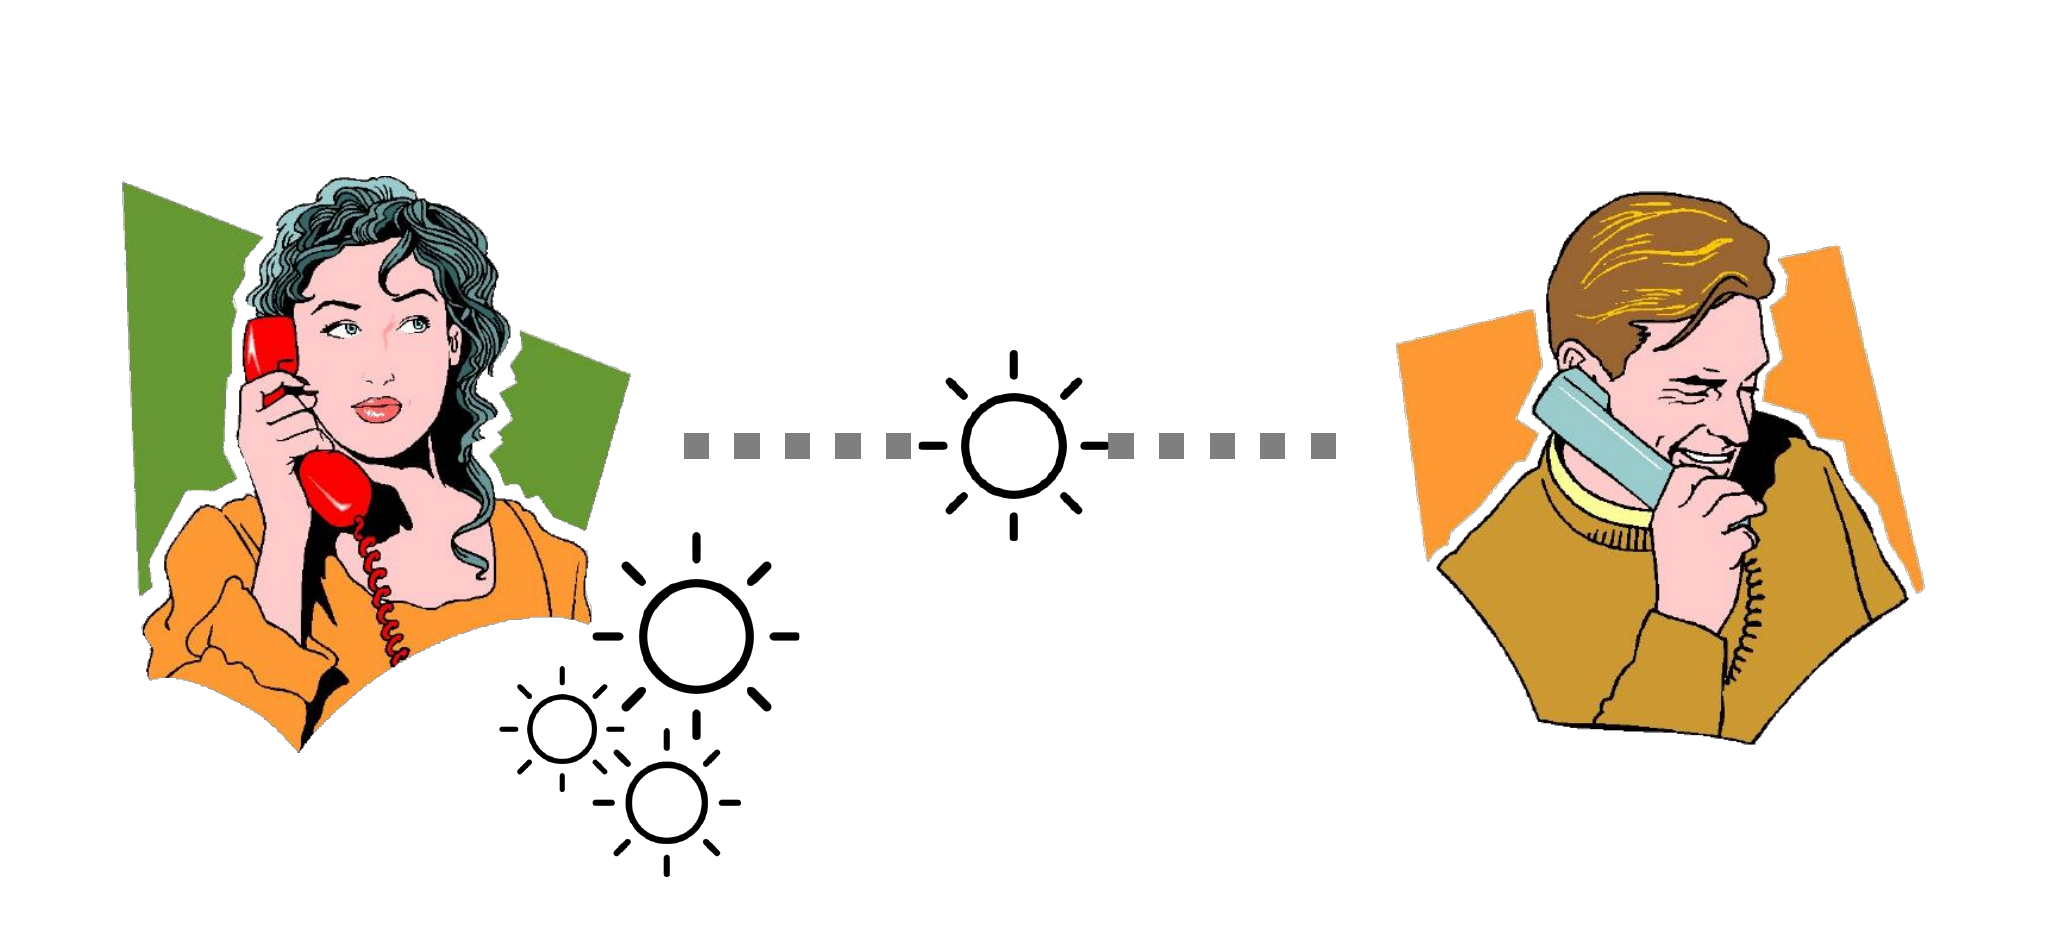
\includegraphics[scale=0.25]{figures/Teleportation/frame_01.png}}
\end{frame}
\begin{frame}
	\makebox[0pt][l]{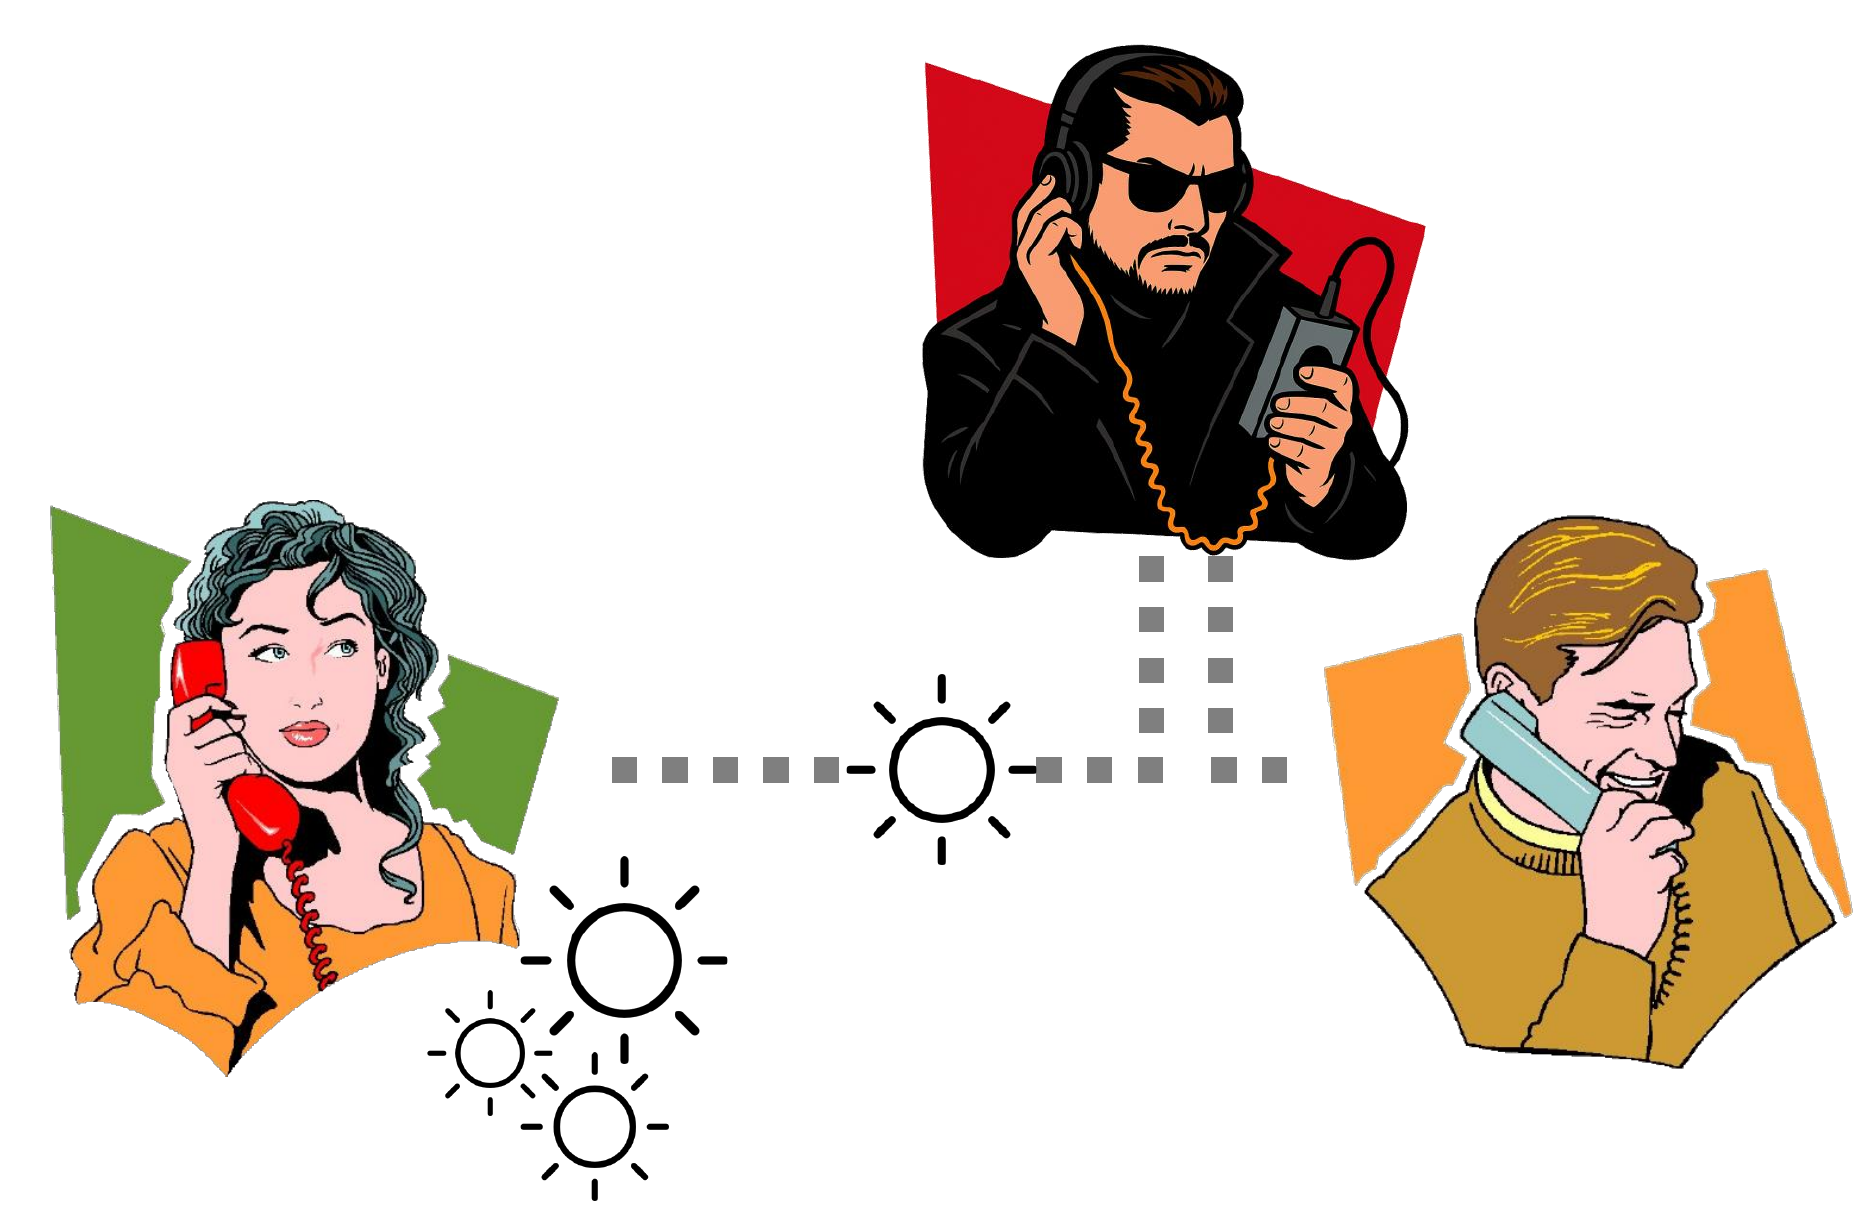
\includegraphics[scale=0.23]{figures/Teleportation/frame_02.png}}
\end{frame}
\begin{frame}
	\vspace{-2em}
	\makebox[0pt][l]{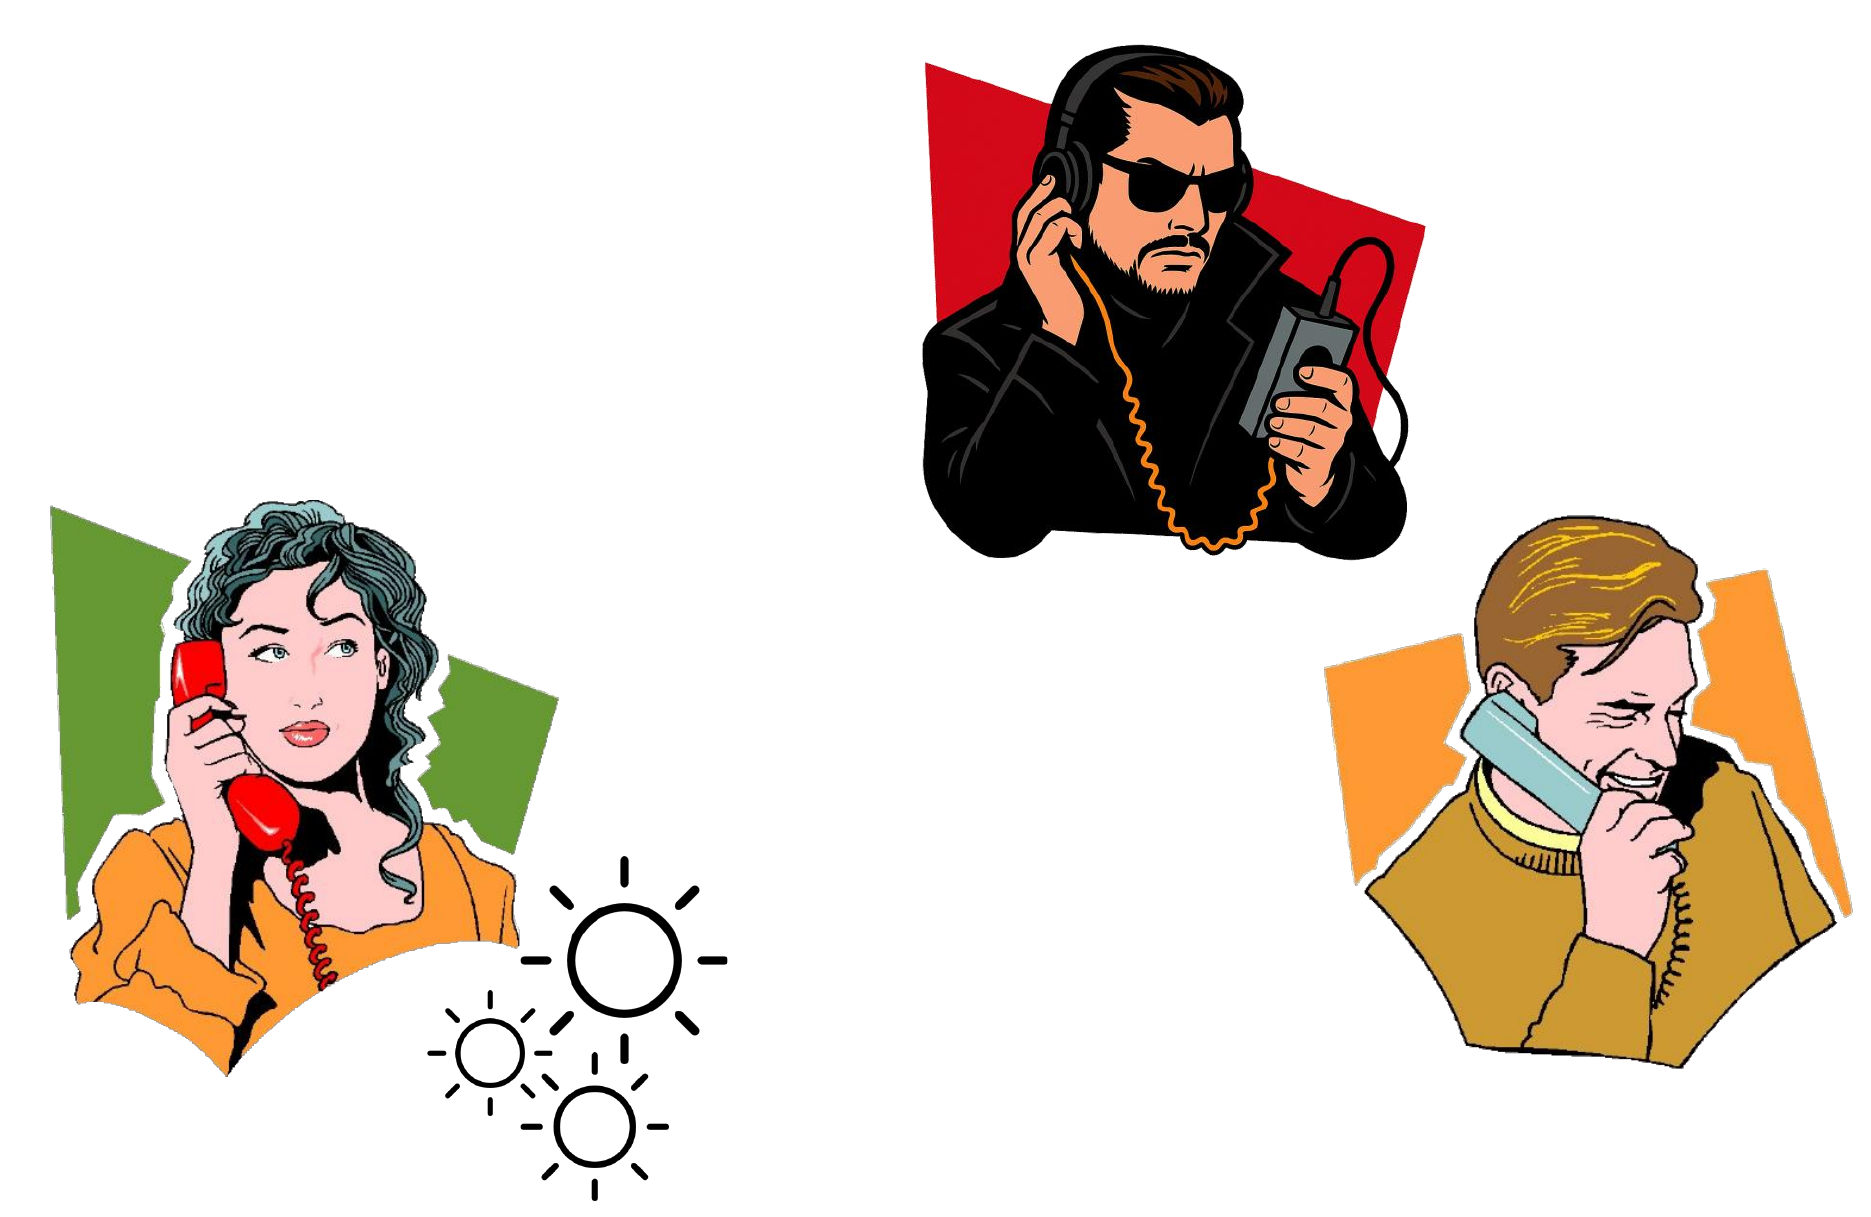
\includegraphics[scale=0.23]{figures/Teleportation/frame_03.png}}
\end{frame}
\begin{frame}
	\vspace{-2em}
	\makebox[0pt][l]{\hspace{-3.5em}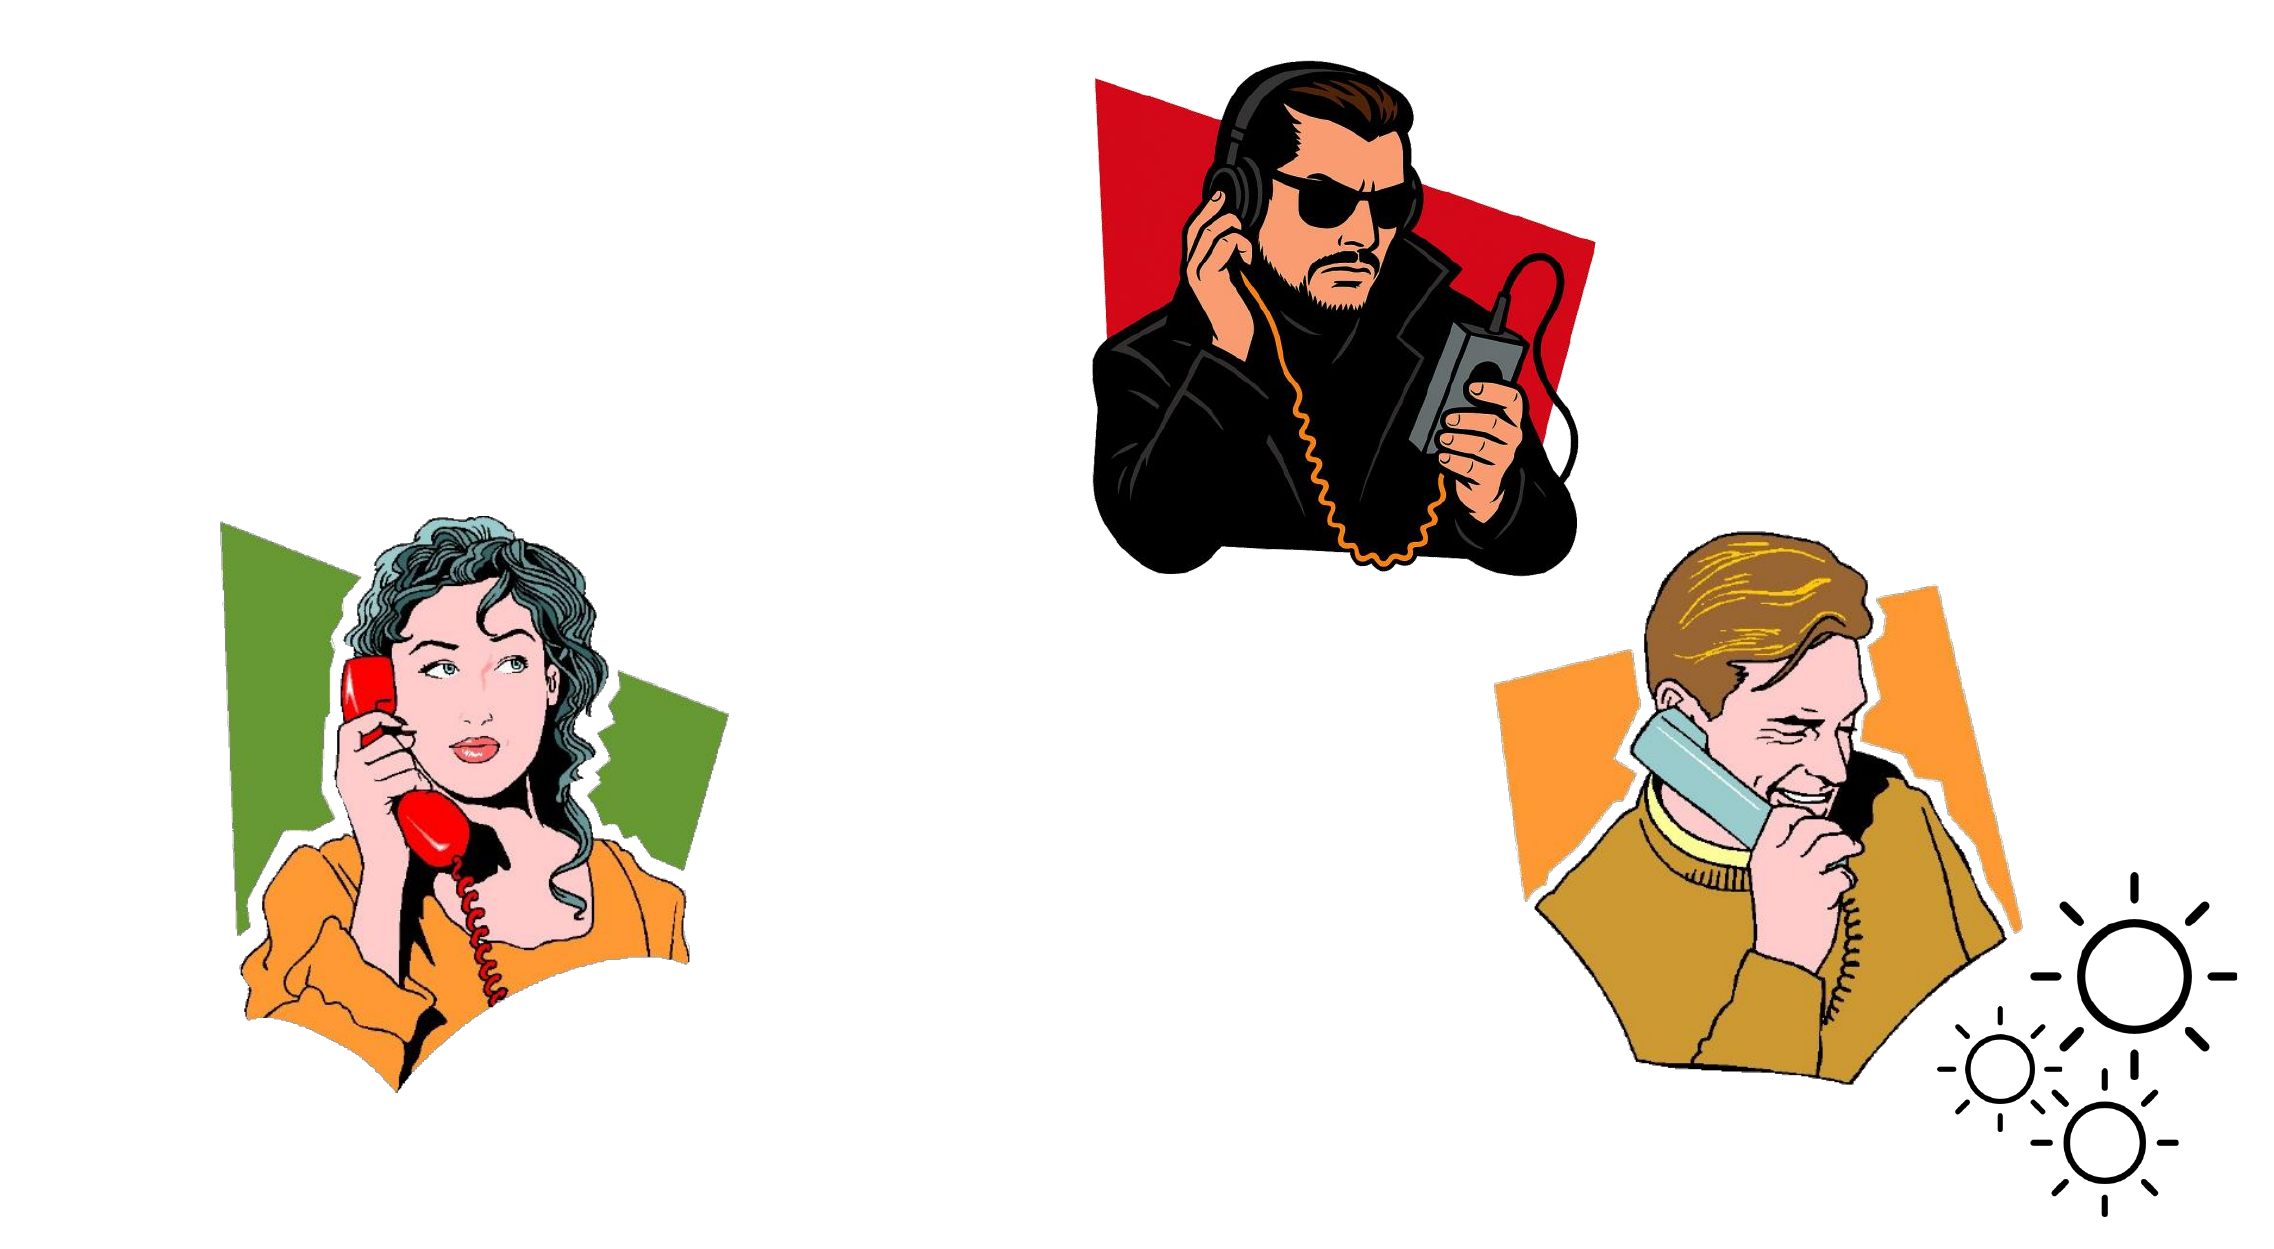
\includegraphics[scale=0.23]{figures/Teleportation/frame_04.png}}
\end{frame}
\begin{frame}
	\vspace{-2em}
	\makebox[0pt][l]{\hspace{-3.5em}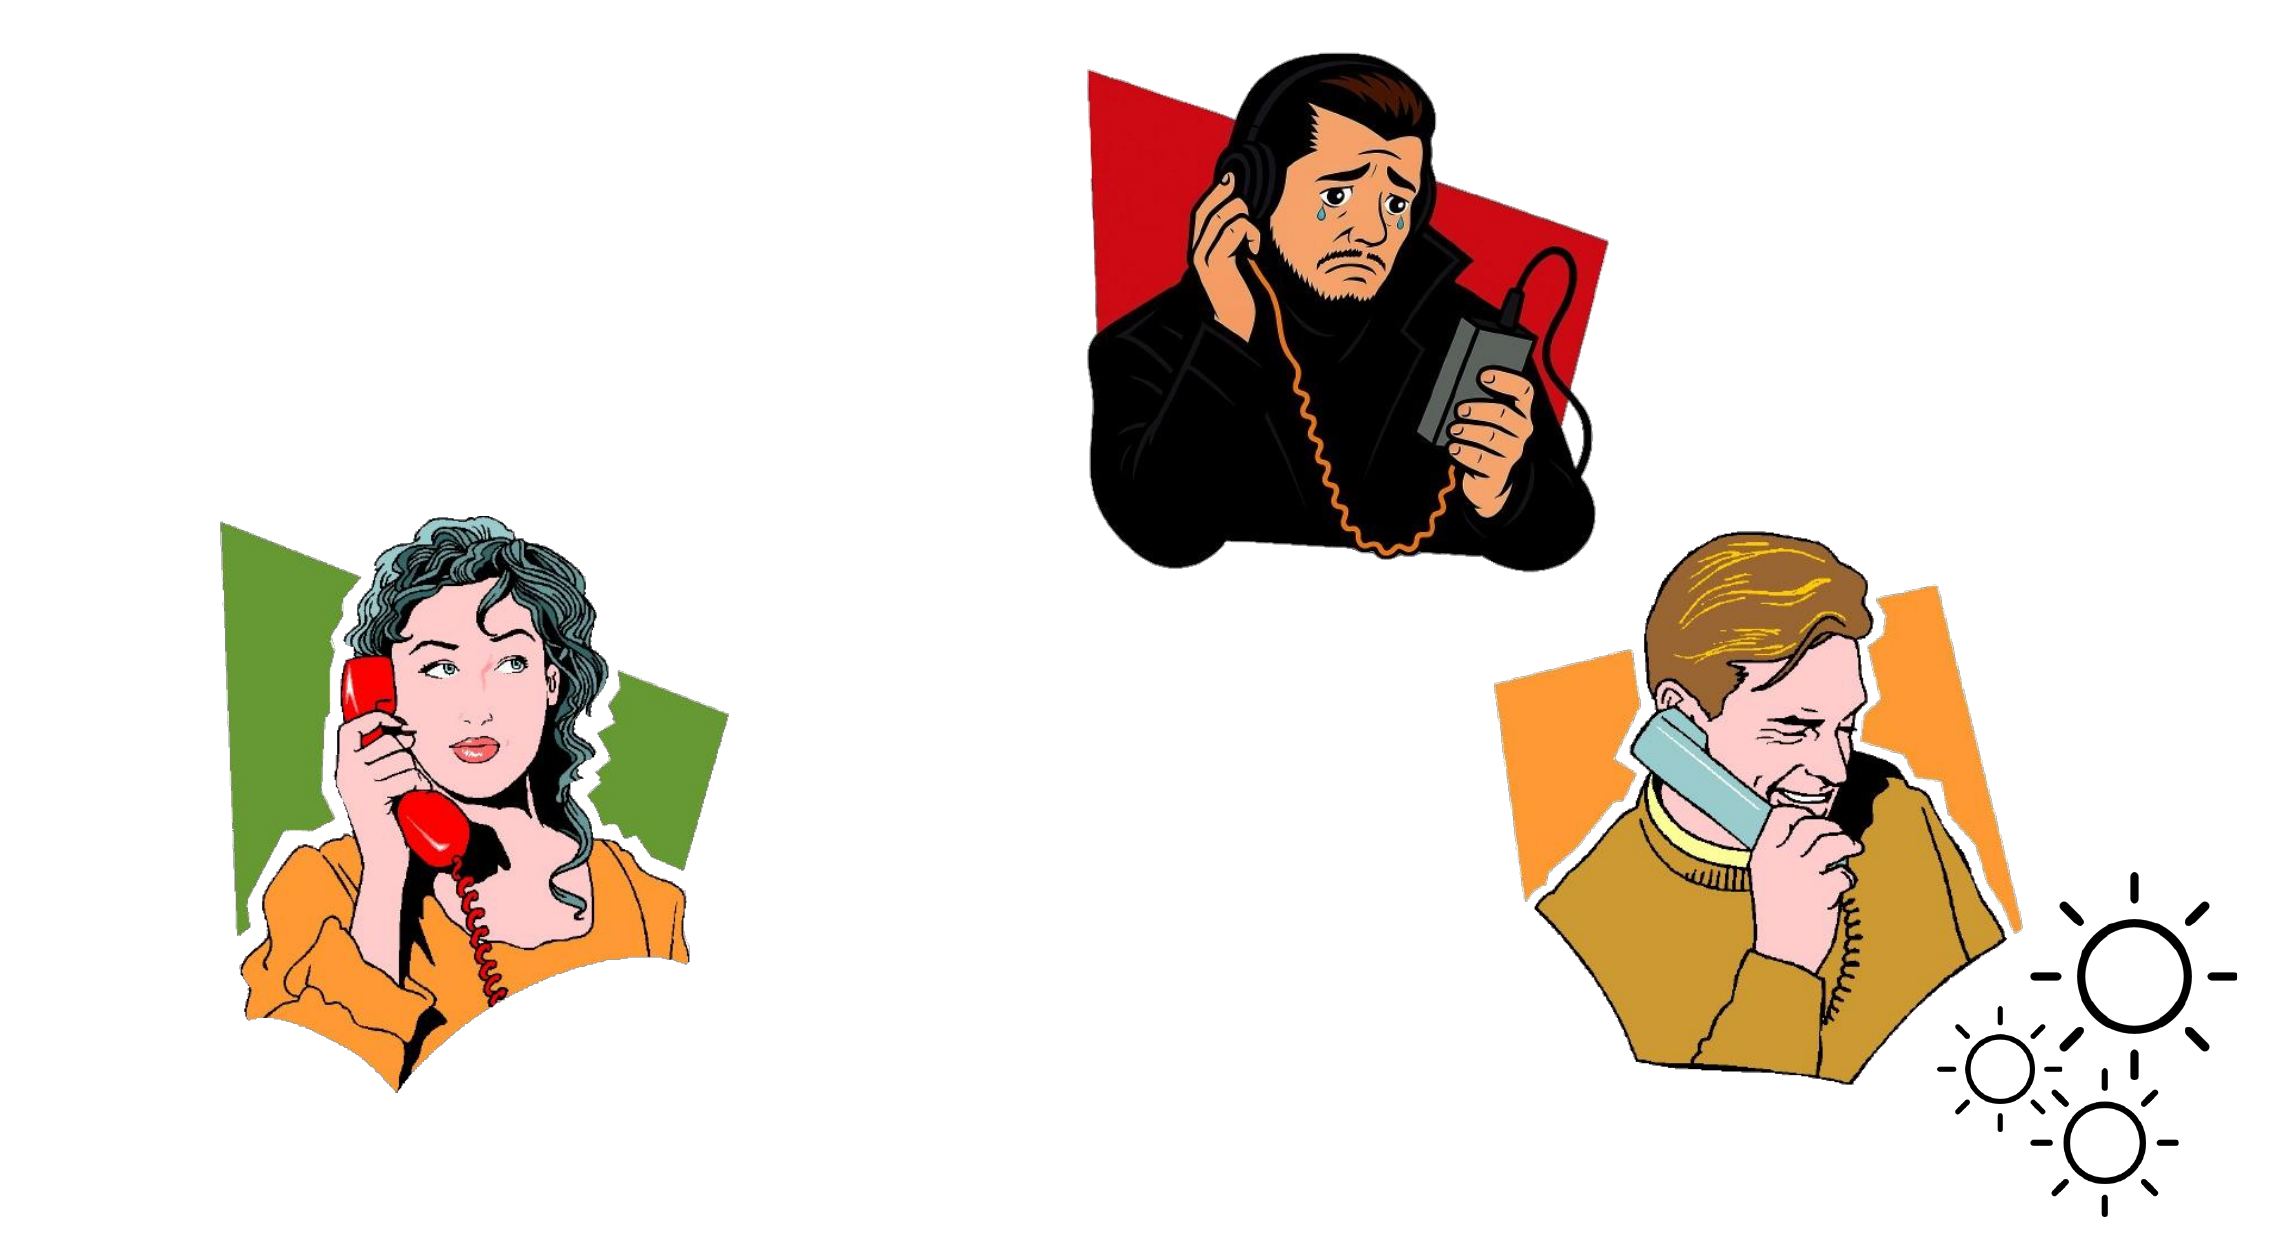
\includegraphics[scale=0.23]{figures/Teleportation/frame_05.png}}
\end{frame}
\begin{frame}
	\makebox[0pt][l]{\hspace{0em}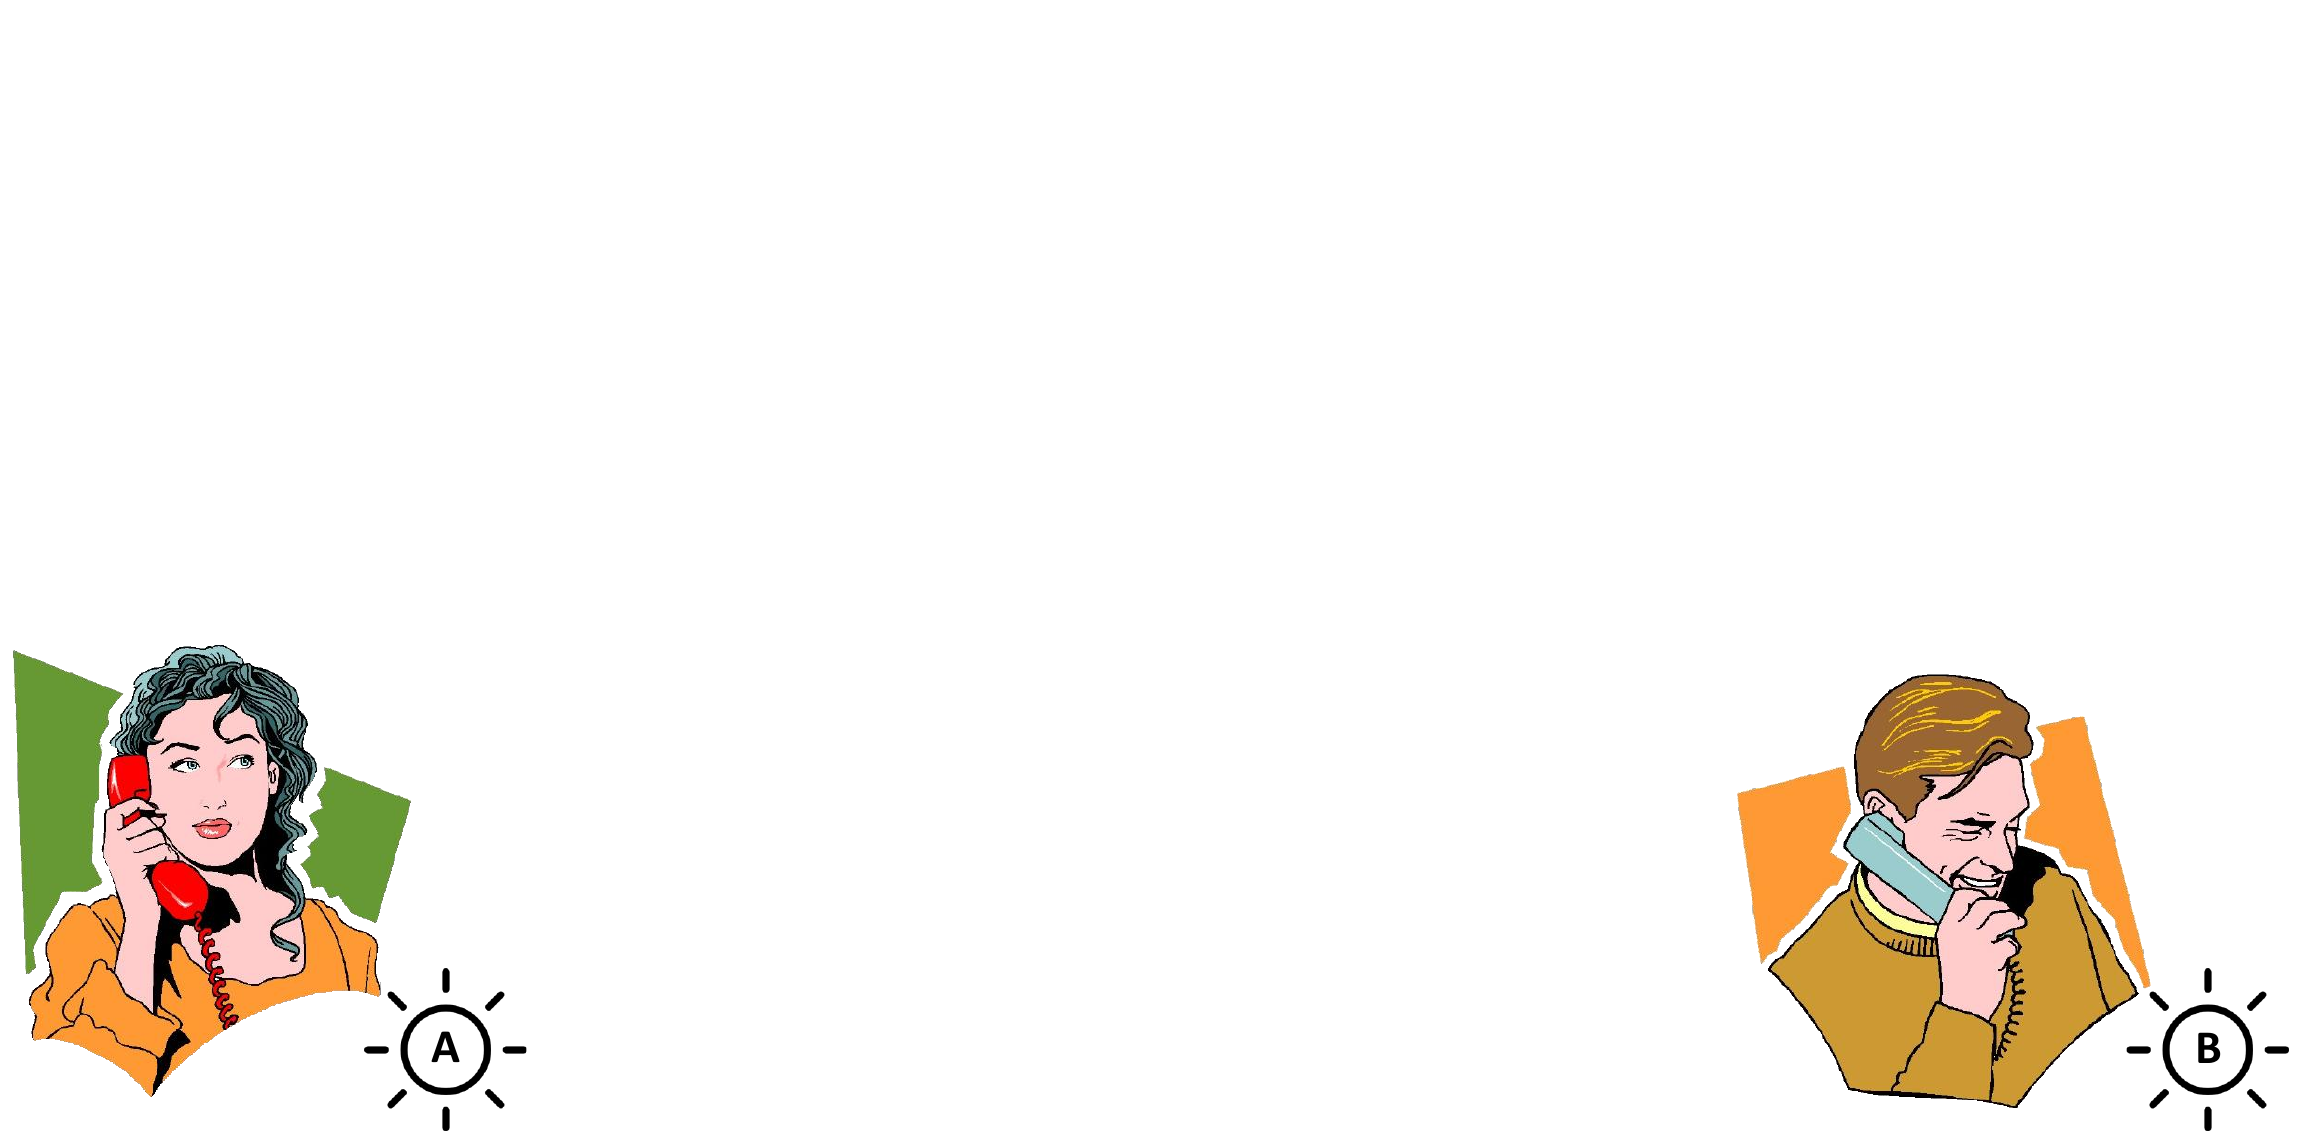
\includegraphics[scale=0.6]{figures/Teleportation/frame_06.png}}
\end{frame}
\begin{frame}
	\makebox[0pt][l]{\hspace{0em}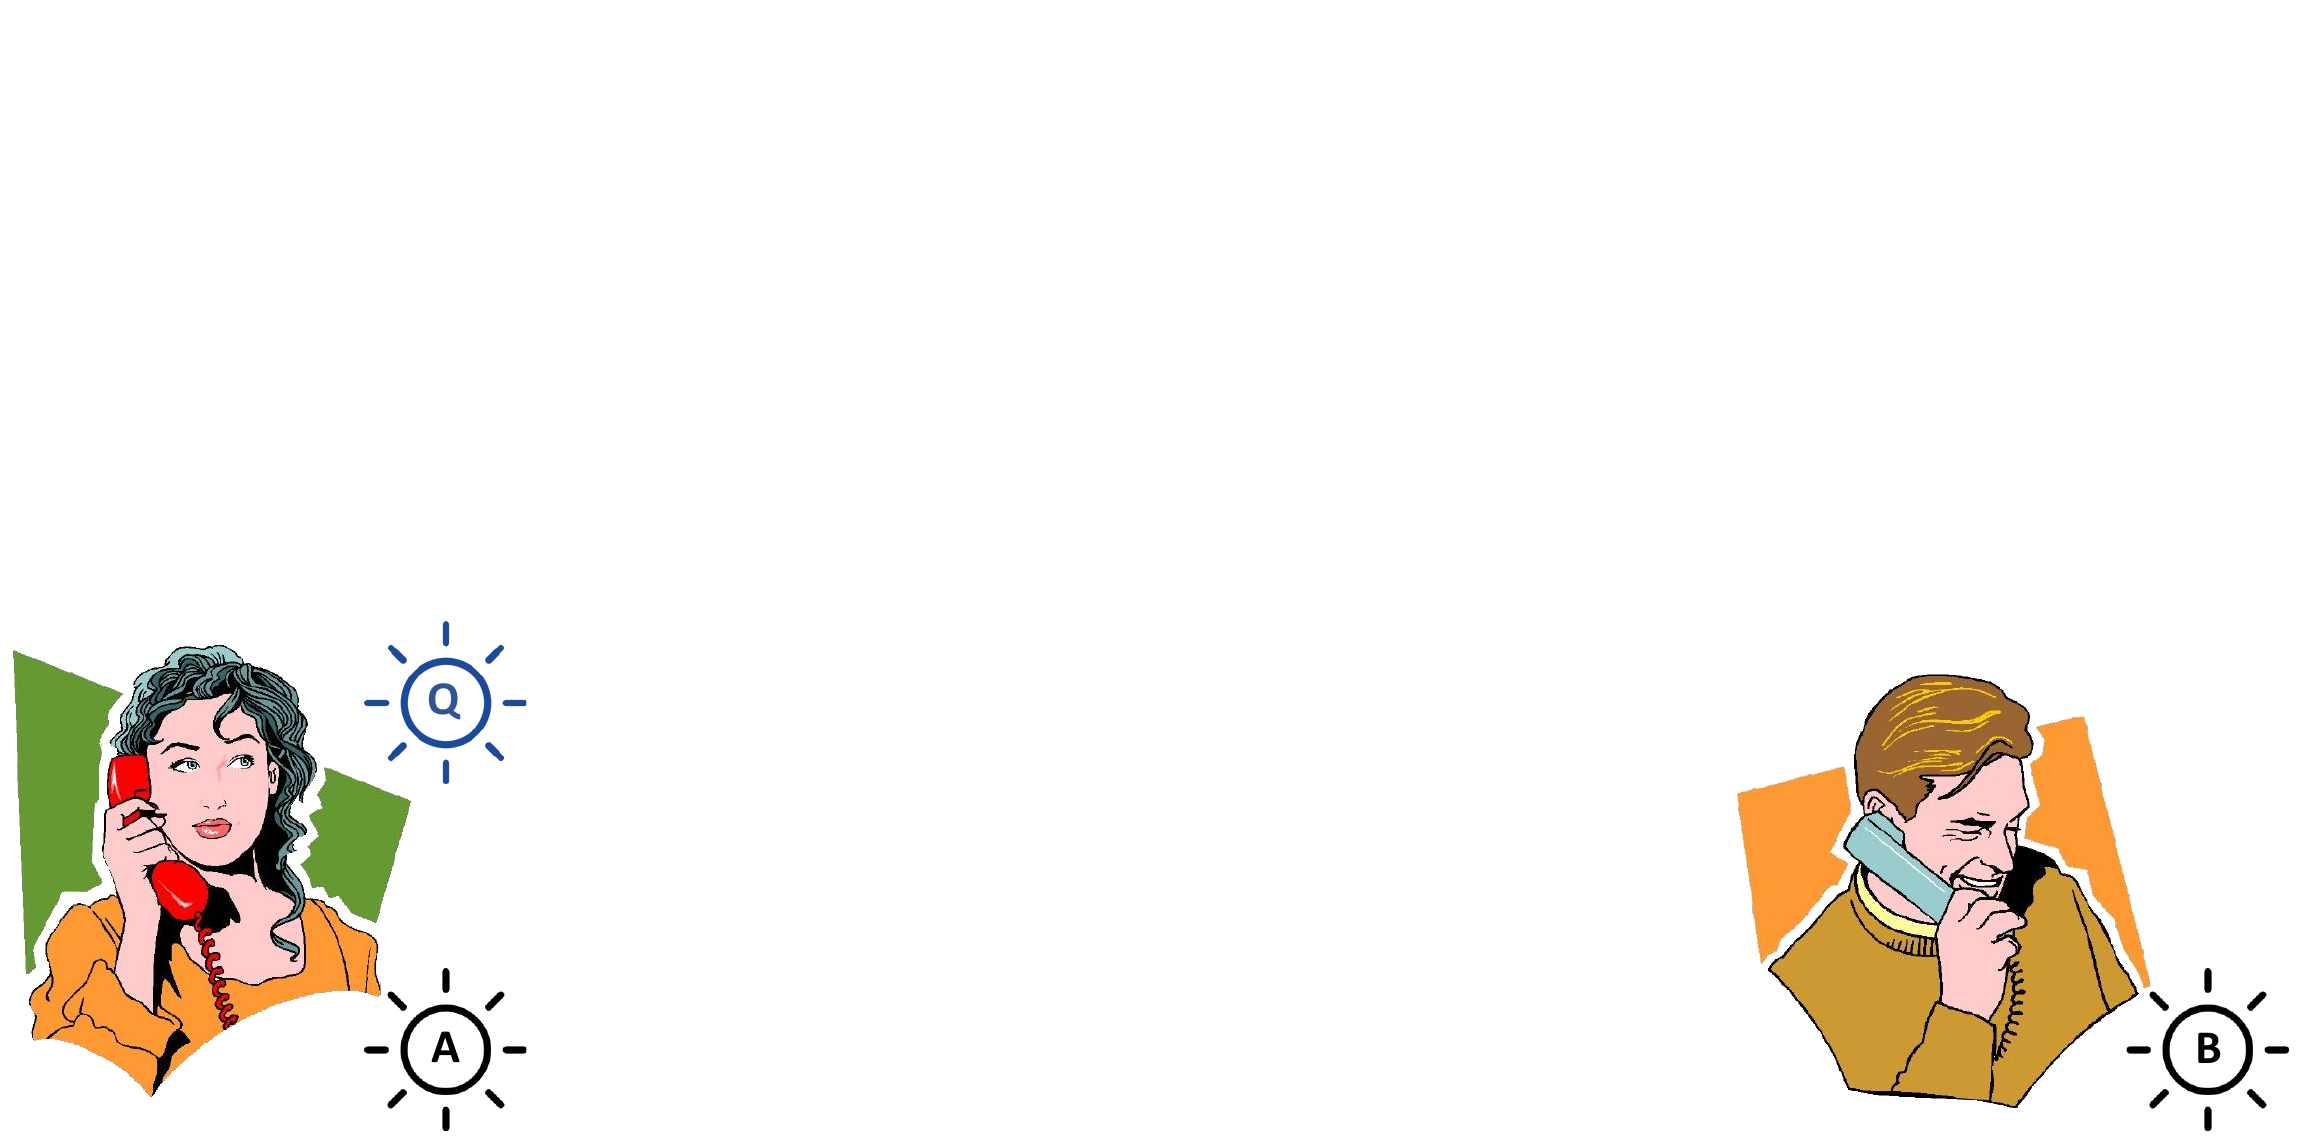
\includegraphics[scale=0.6]{figures/Teleportation/frame_07.png}}
\end{frame}
\begin{frame}
	\makebox[0pt][l]{\hspace{0em}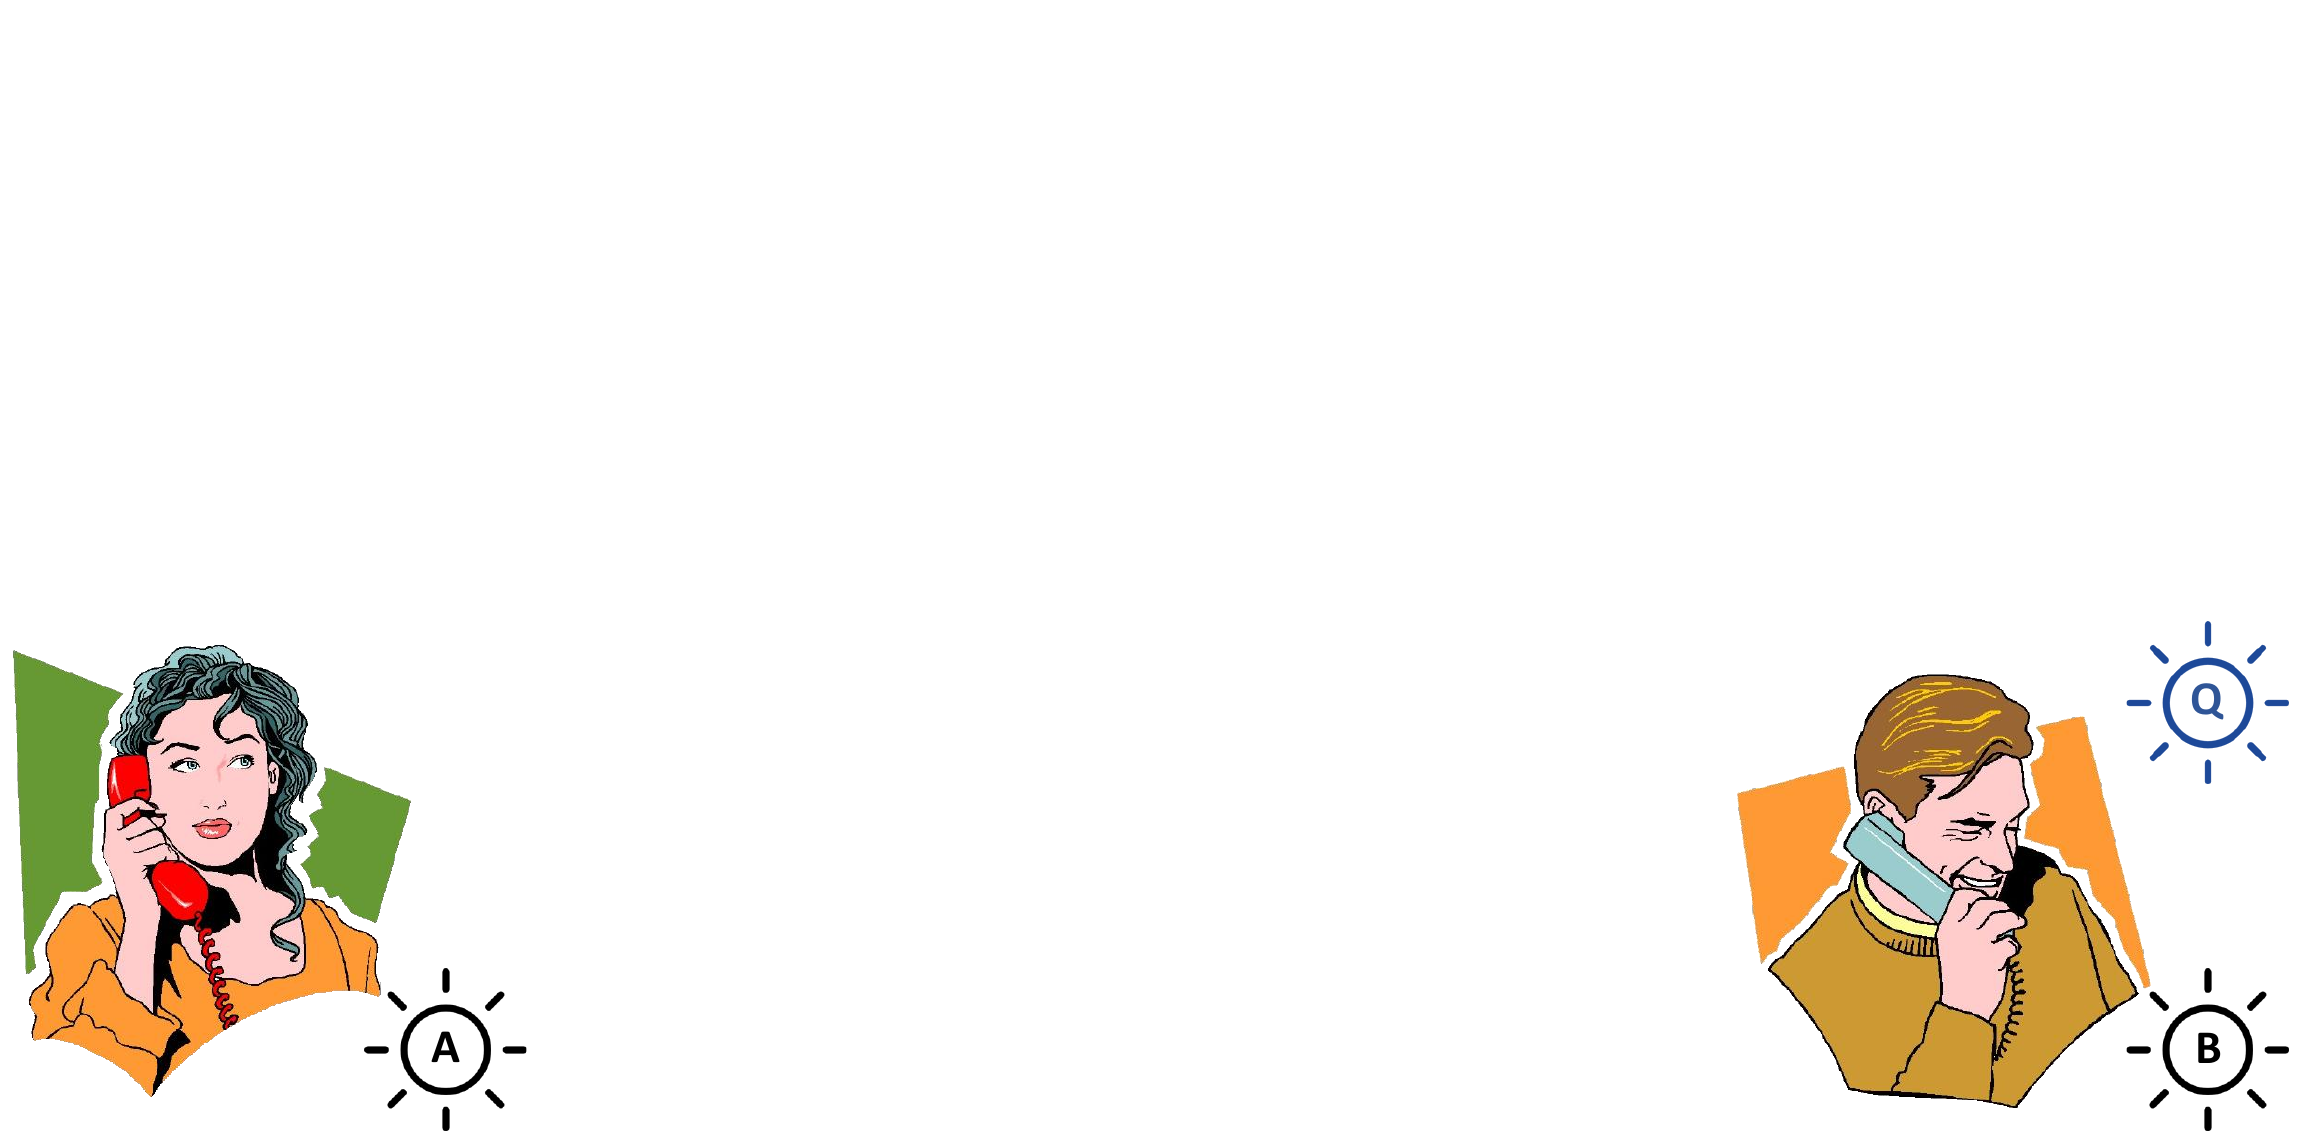
\includegraphics[scale=0.6]{figures/Teleportation/frame_08.png}}
\end{frame}
\begin{frame}
	\makebox[0pt][l]{\hspace{-2em}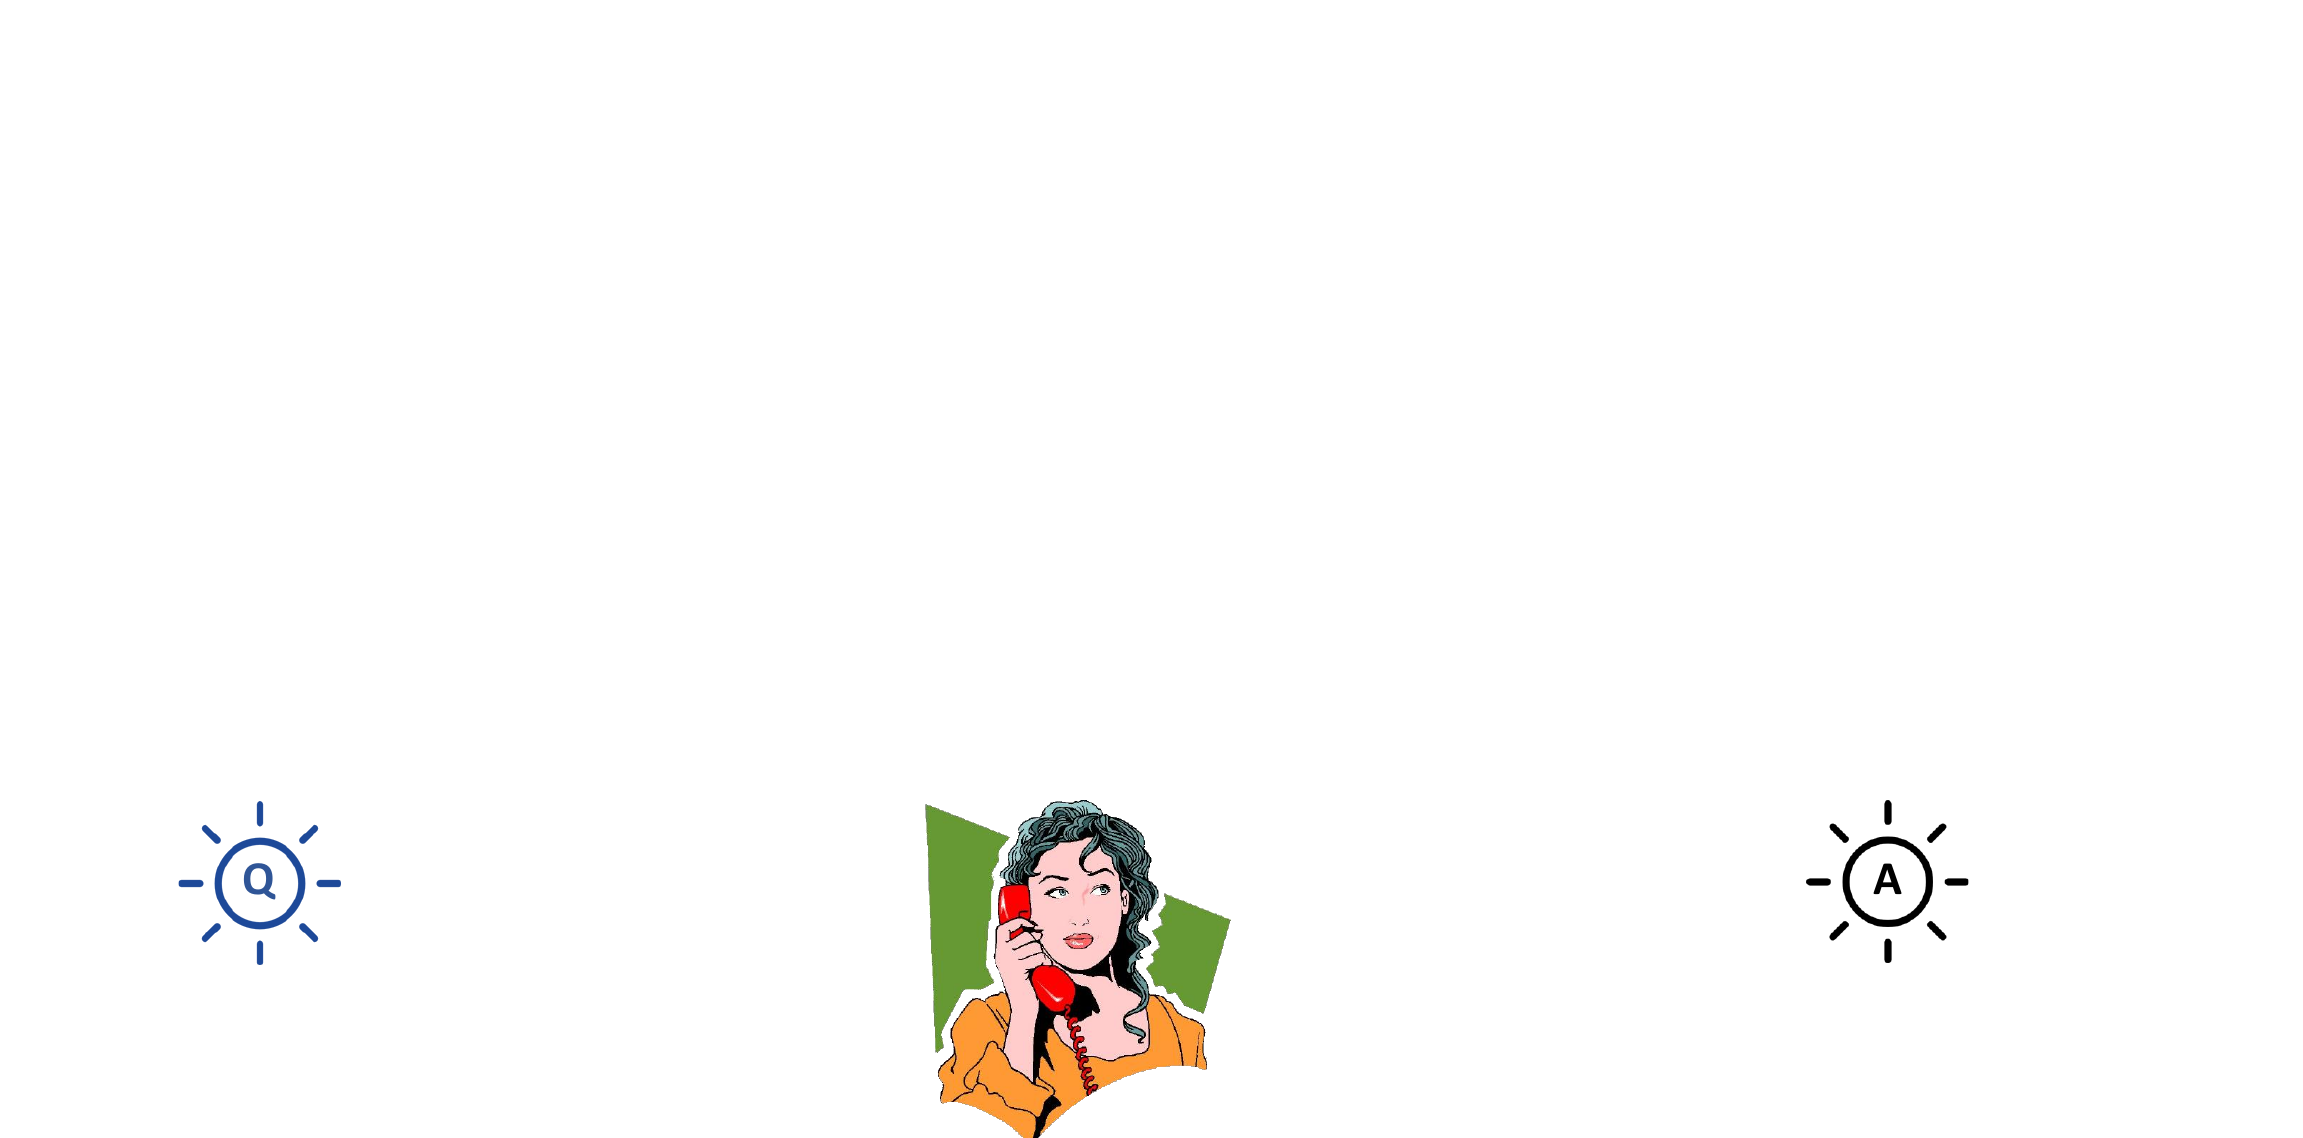
\includegraphics[scale=0.75]{figures/Teleportation/frame_09.png}}
\end{frame}
\begin{frame}
	\makebox[0pt][l]{\hspace{-2em}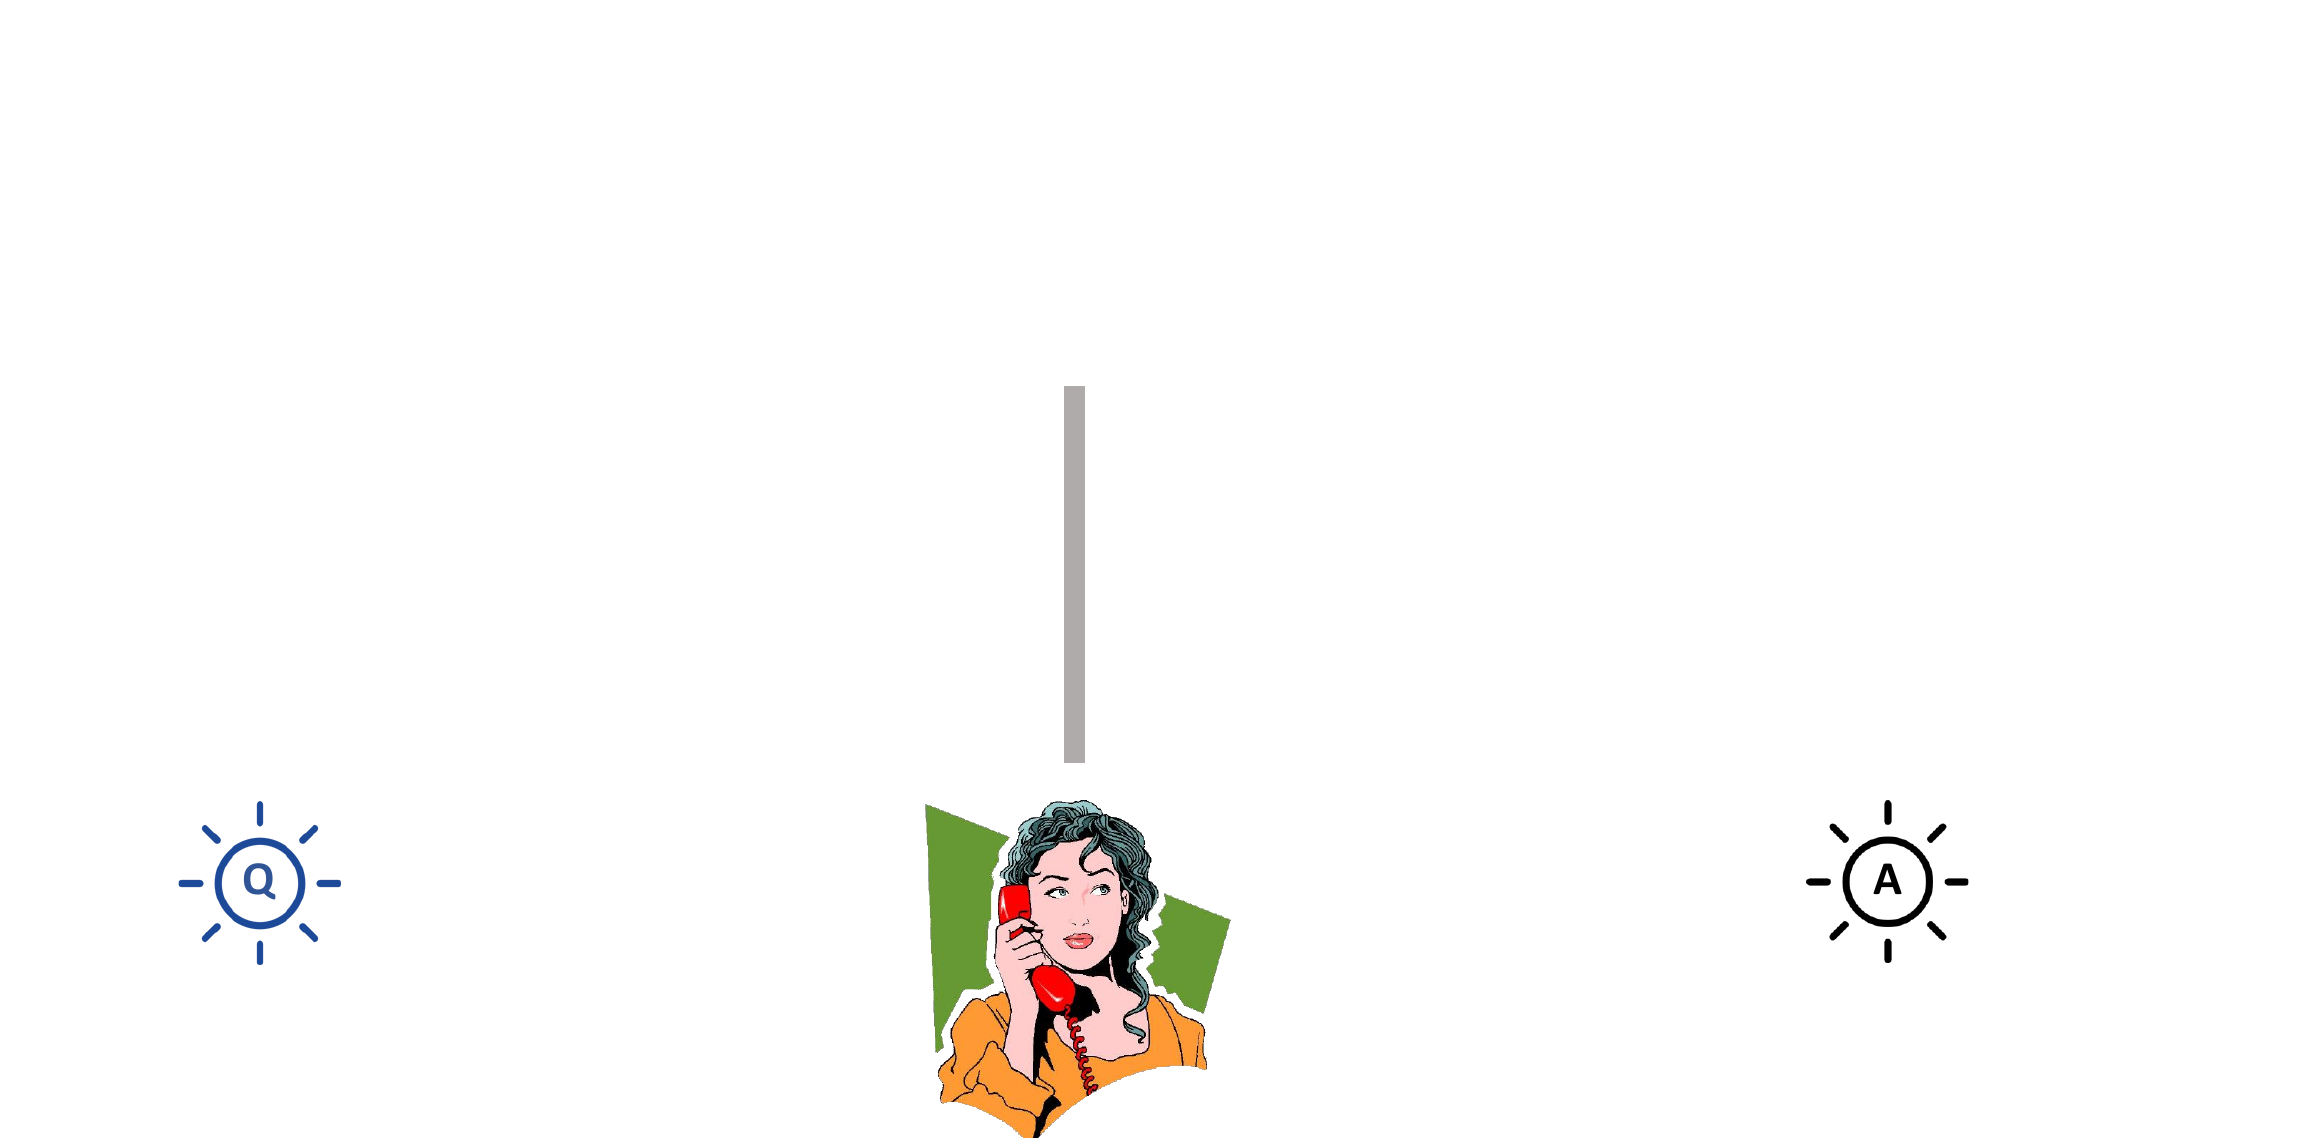
\includegraphics[scale=0.75]{figures/Teleportation/frame_10.png}}
\end{frame}
\begin{frame}
	\makebox[0pt][l]{\hspace{-2em}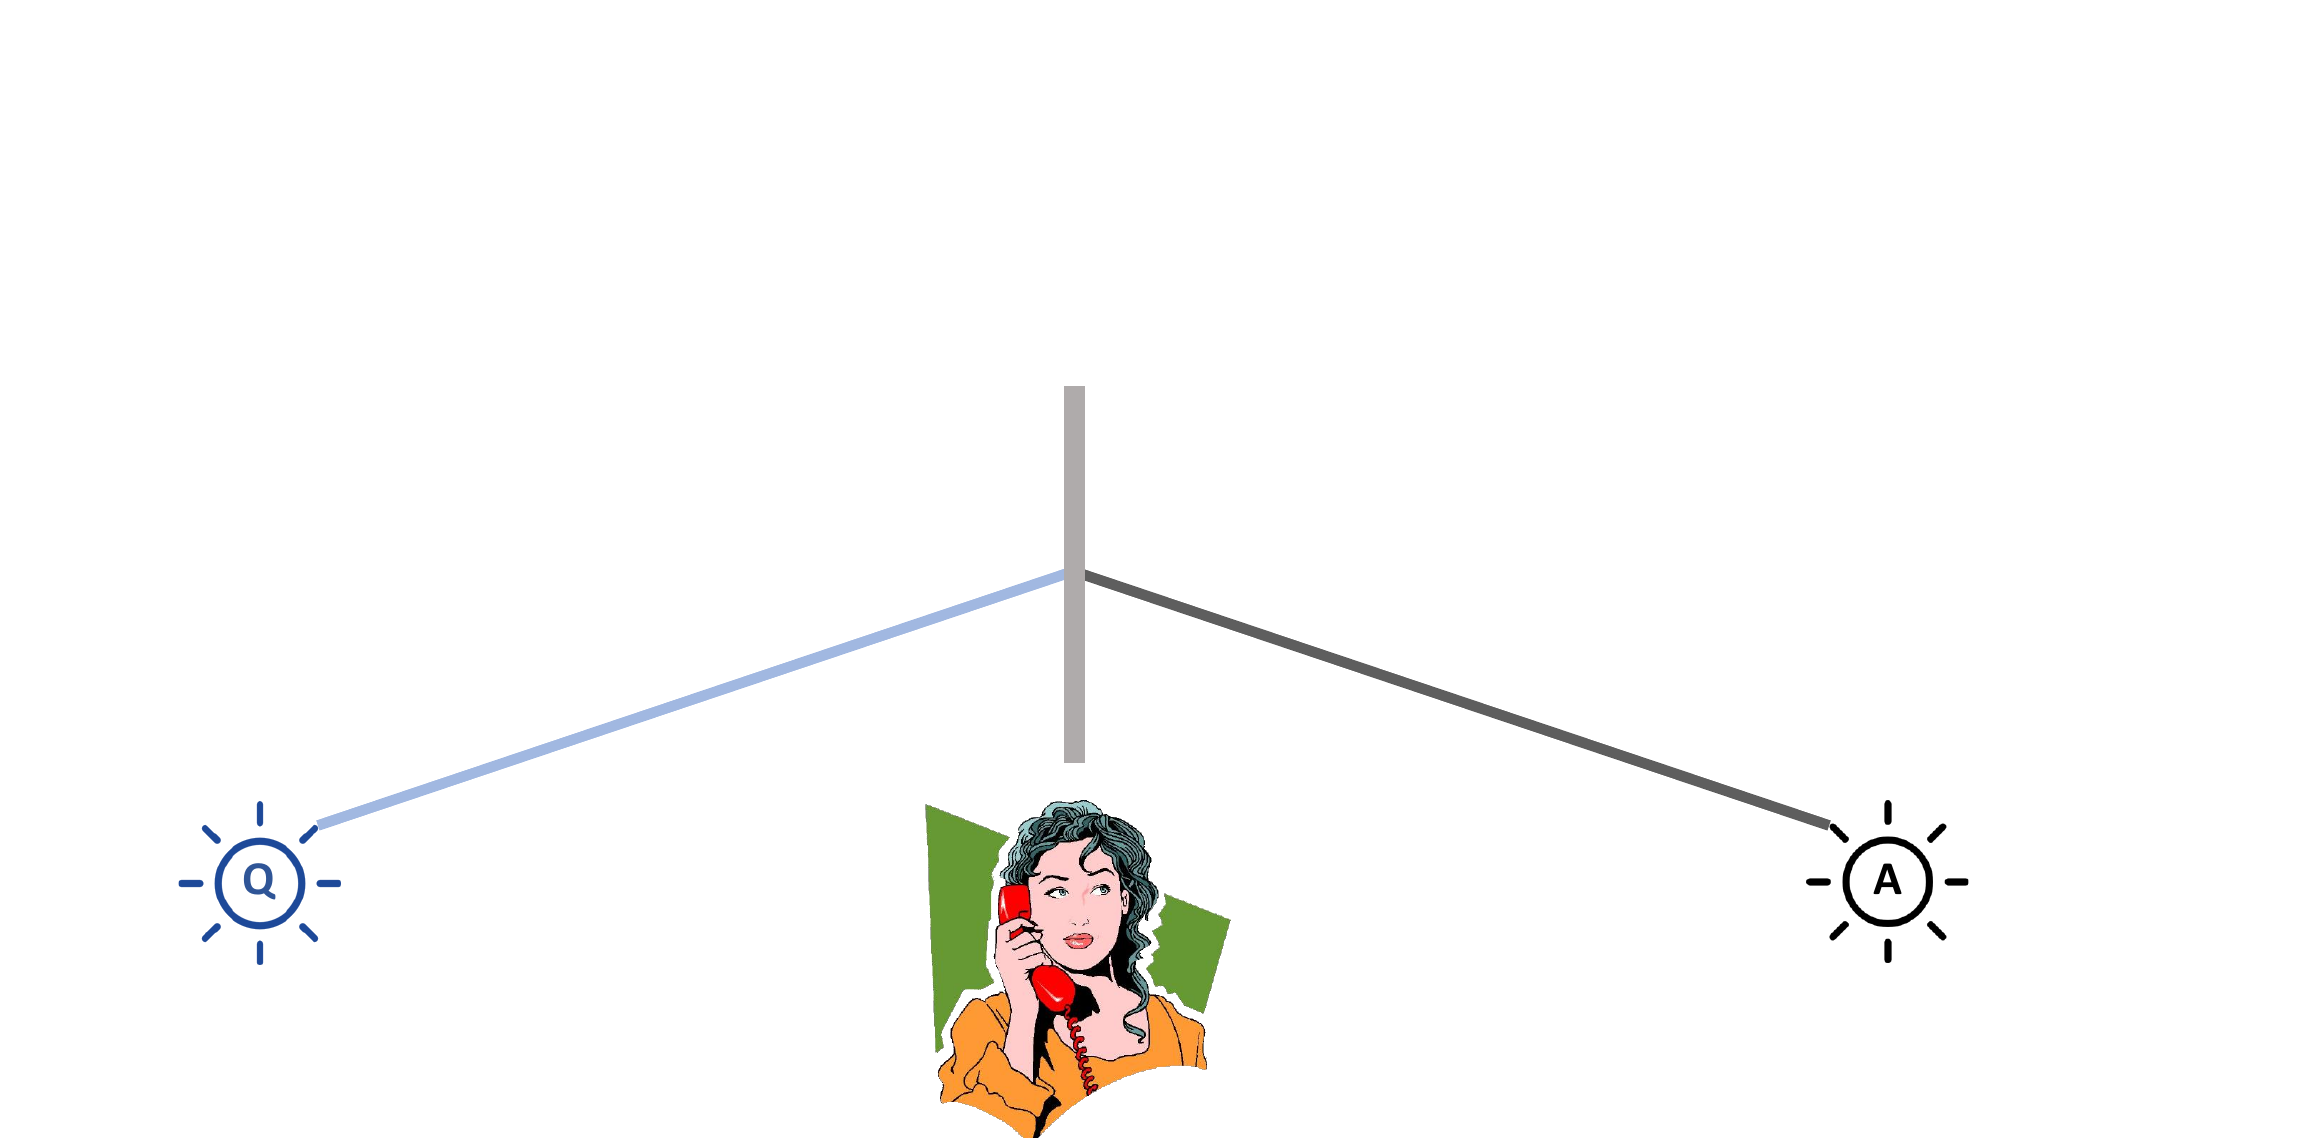
\includegraphics[scale=0.75]{figures/Teleportation/frame_11.png}}
\end{frame}

\begin{frame}
	\frametitle{Halbdurchl{\"a}ssiger Spiegel}
		\begin{columns}
		\begin{column}{0.64\linewidth}
			-- Teilt ein einfallendes Photon mit $50\%$\\
				\hspace{0.5em} Wahrscheinlichkeit in zwei Ausgänge auf: \\
				\hspace{0.5em} \textbf{Transmission} oder \textbf{Reflexion}.\\
			--  In der Quantenmechanik bedeutet das:\\
				\hspace{0.5em} Das Photon geht in eine \textbf{{\"U}berlagerung} \\
				\hspace{0.5em} beider Wege – es ist \enquote{gleichzeitig} reflektiert \\
				\hspace{0.5em} und durchgelassen.\\
		\end{column}
		\begin{column}{0.34\linewidth}
			\img{1.0\linewidth}{Kommunikation/half_passing_mirror}{half_passing_mirror}{Photonen am halbdurchl{\"a}ssigen Spiegel}{Photonen am halbdurchl{\"a}ssigen Spiegel}
		\end{column}
	\end{columns}
\end{frame}

\begin{frame}
	\frametitle{Hong–Ou–Mandel-Effekt}
	\begin{columns}
		\begin{column}{0.33\linewidth}
			\img{0.9\linewidth}{Teleportation/beam_splitter}{hom_effect}{Beam Splitter}{Beam Splitter}
		\end{column}
		\begin{column}{0.66\linewidth}
			\img{1.0\linewidth}{Teleportation/hom_effect}{hom_effect}{HOM Effekt}{HOM Effekt}
		\end{column}
	\end{columns}
	Dieses Verhalten macht den Beam Splitter zur zentralen Komponente für \textbf{Bell-Messungen}, Quanten-Interferometer und \textbf{Quanten-Teleportation}.
\end{frame}

\begin{frame}
	\frametitle{Bell States}
	\begin{align*}
		\lvert \Phi^+ \rangle &= \frac{1}{\sqrt{2}} \left( \lvert 0 \rangle_A \otimes \lvert 0 \rangle_B + \lvert 1 \rangle_A \otimes \lvert 1 \rangle_B \right) \\
		\lvert \Phi^- \rangle &= \frac{1}{\sqrt{2}} \left( \lvert 0 \rangle_A \otimes \lvert 0 \rangle_B - \lvert 1 \rangle_A \otimes \lvert 1 \rangle_B \right) \\
		\lvert \Psi^+ \rangle &= \frac{1}{\sqrt{2}} \left( \lvert 0 \rangle_A \otimes \lvert 1 \rangle_B + \lvert 1 \rangle_A \otimes \lvert 0 \rangle_B \right) \\
		\lvert \Psi^- \rangle &= \frac{1}{\sqrt{2}} \left( \lvert 0 \rangle_A \otimes \lvert 1 \rangle_B - \lvert 1 \rangle_A \otimes \lvert 0 \rangle_B \right)
	\end{align*}
\end{frame}

\begin{frame}
	\makebox[0pt][l]{\hspace{-2em}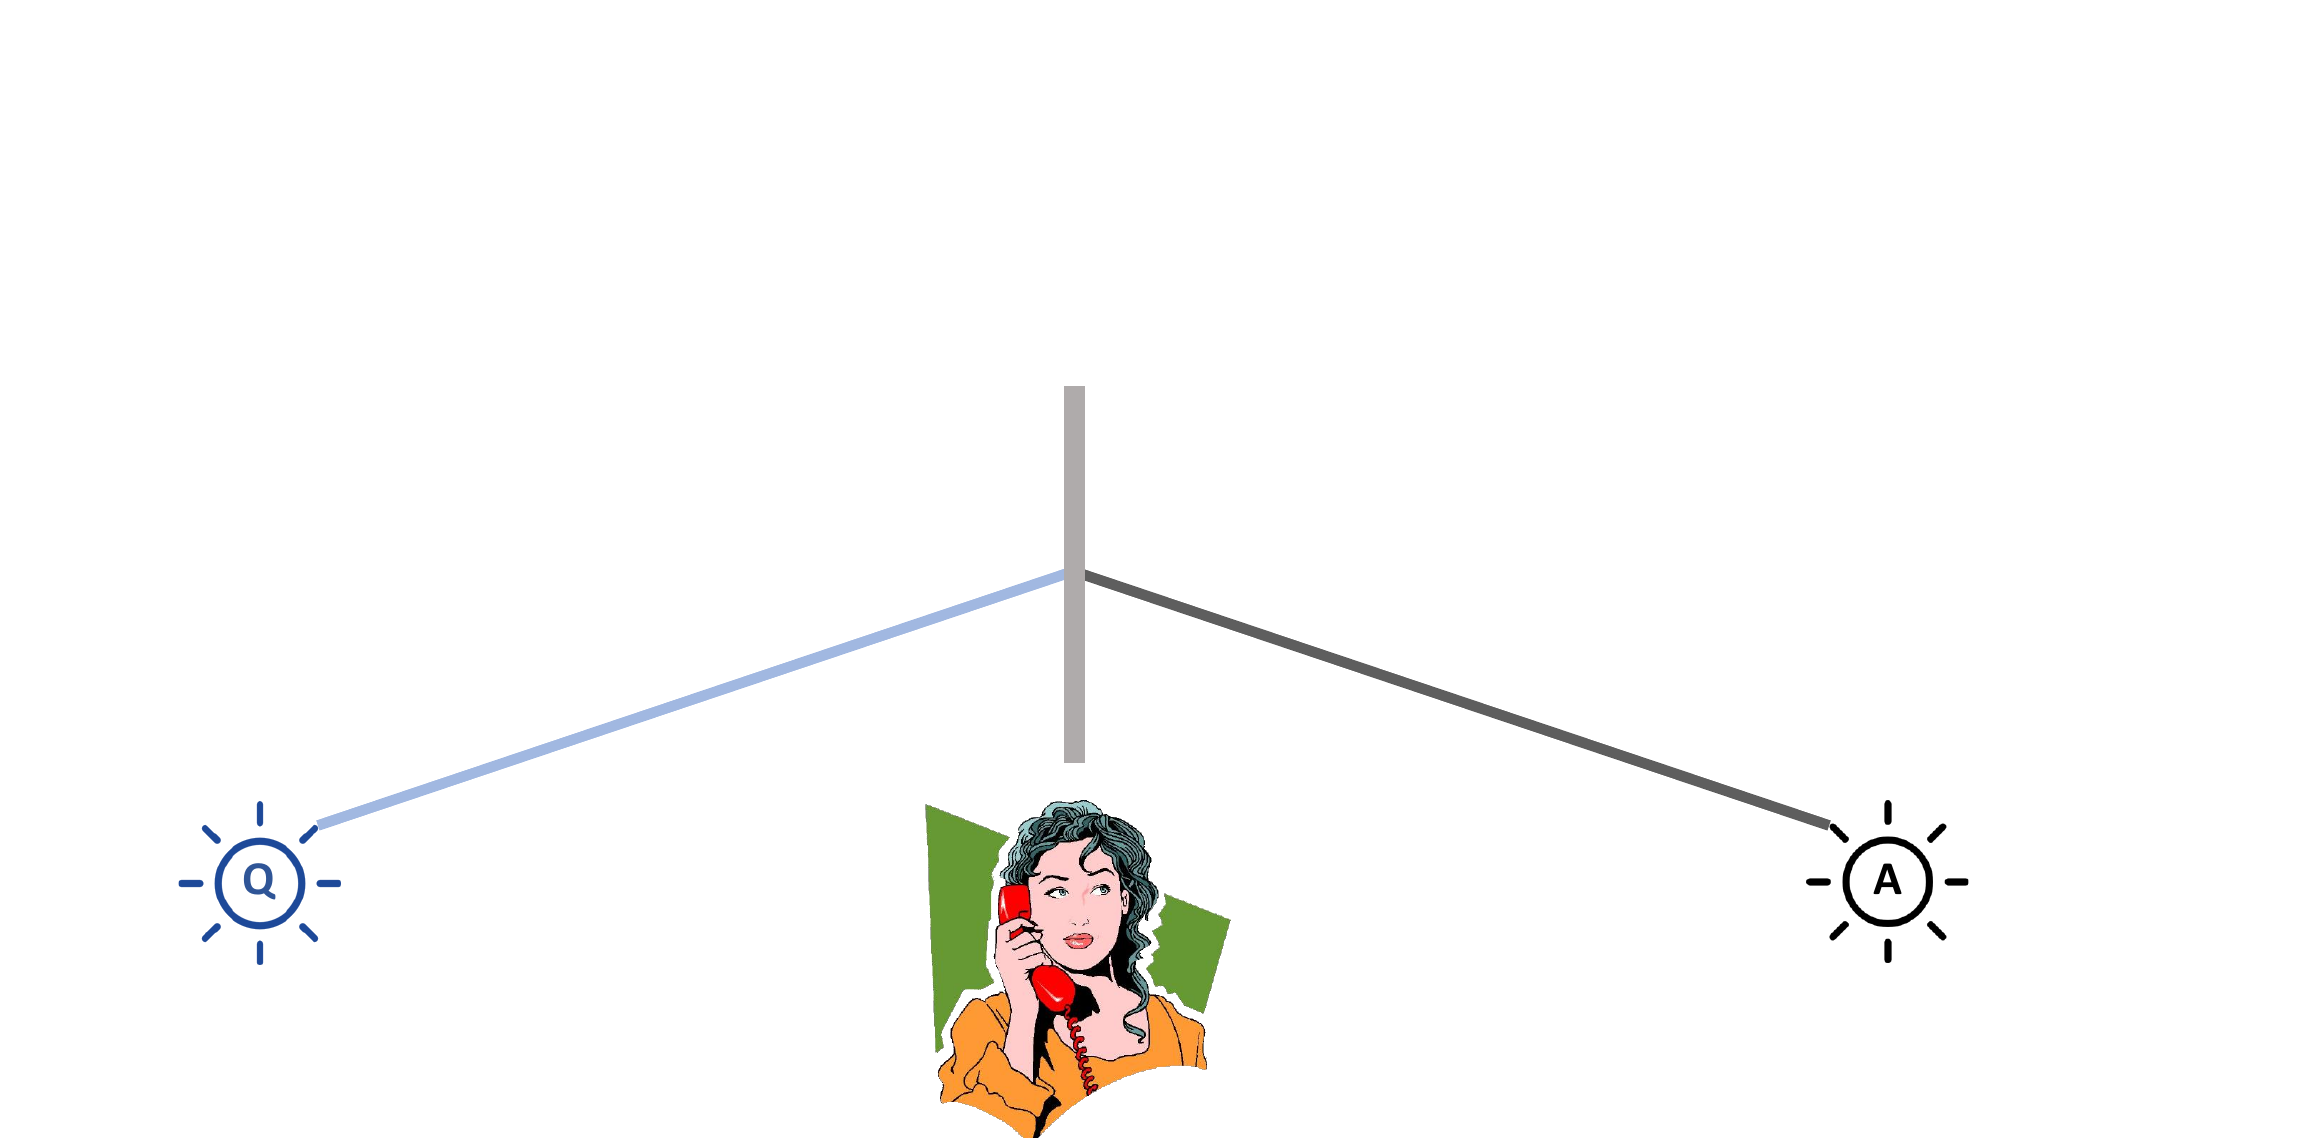
\includegraphics[scale=0.75]{figures/Teleportation/frame_11.png}}
\end{frame}

\begin{frame}
	\makebox[0pt][l]{\hspace{-2em}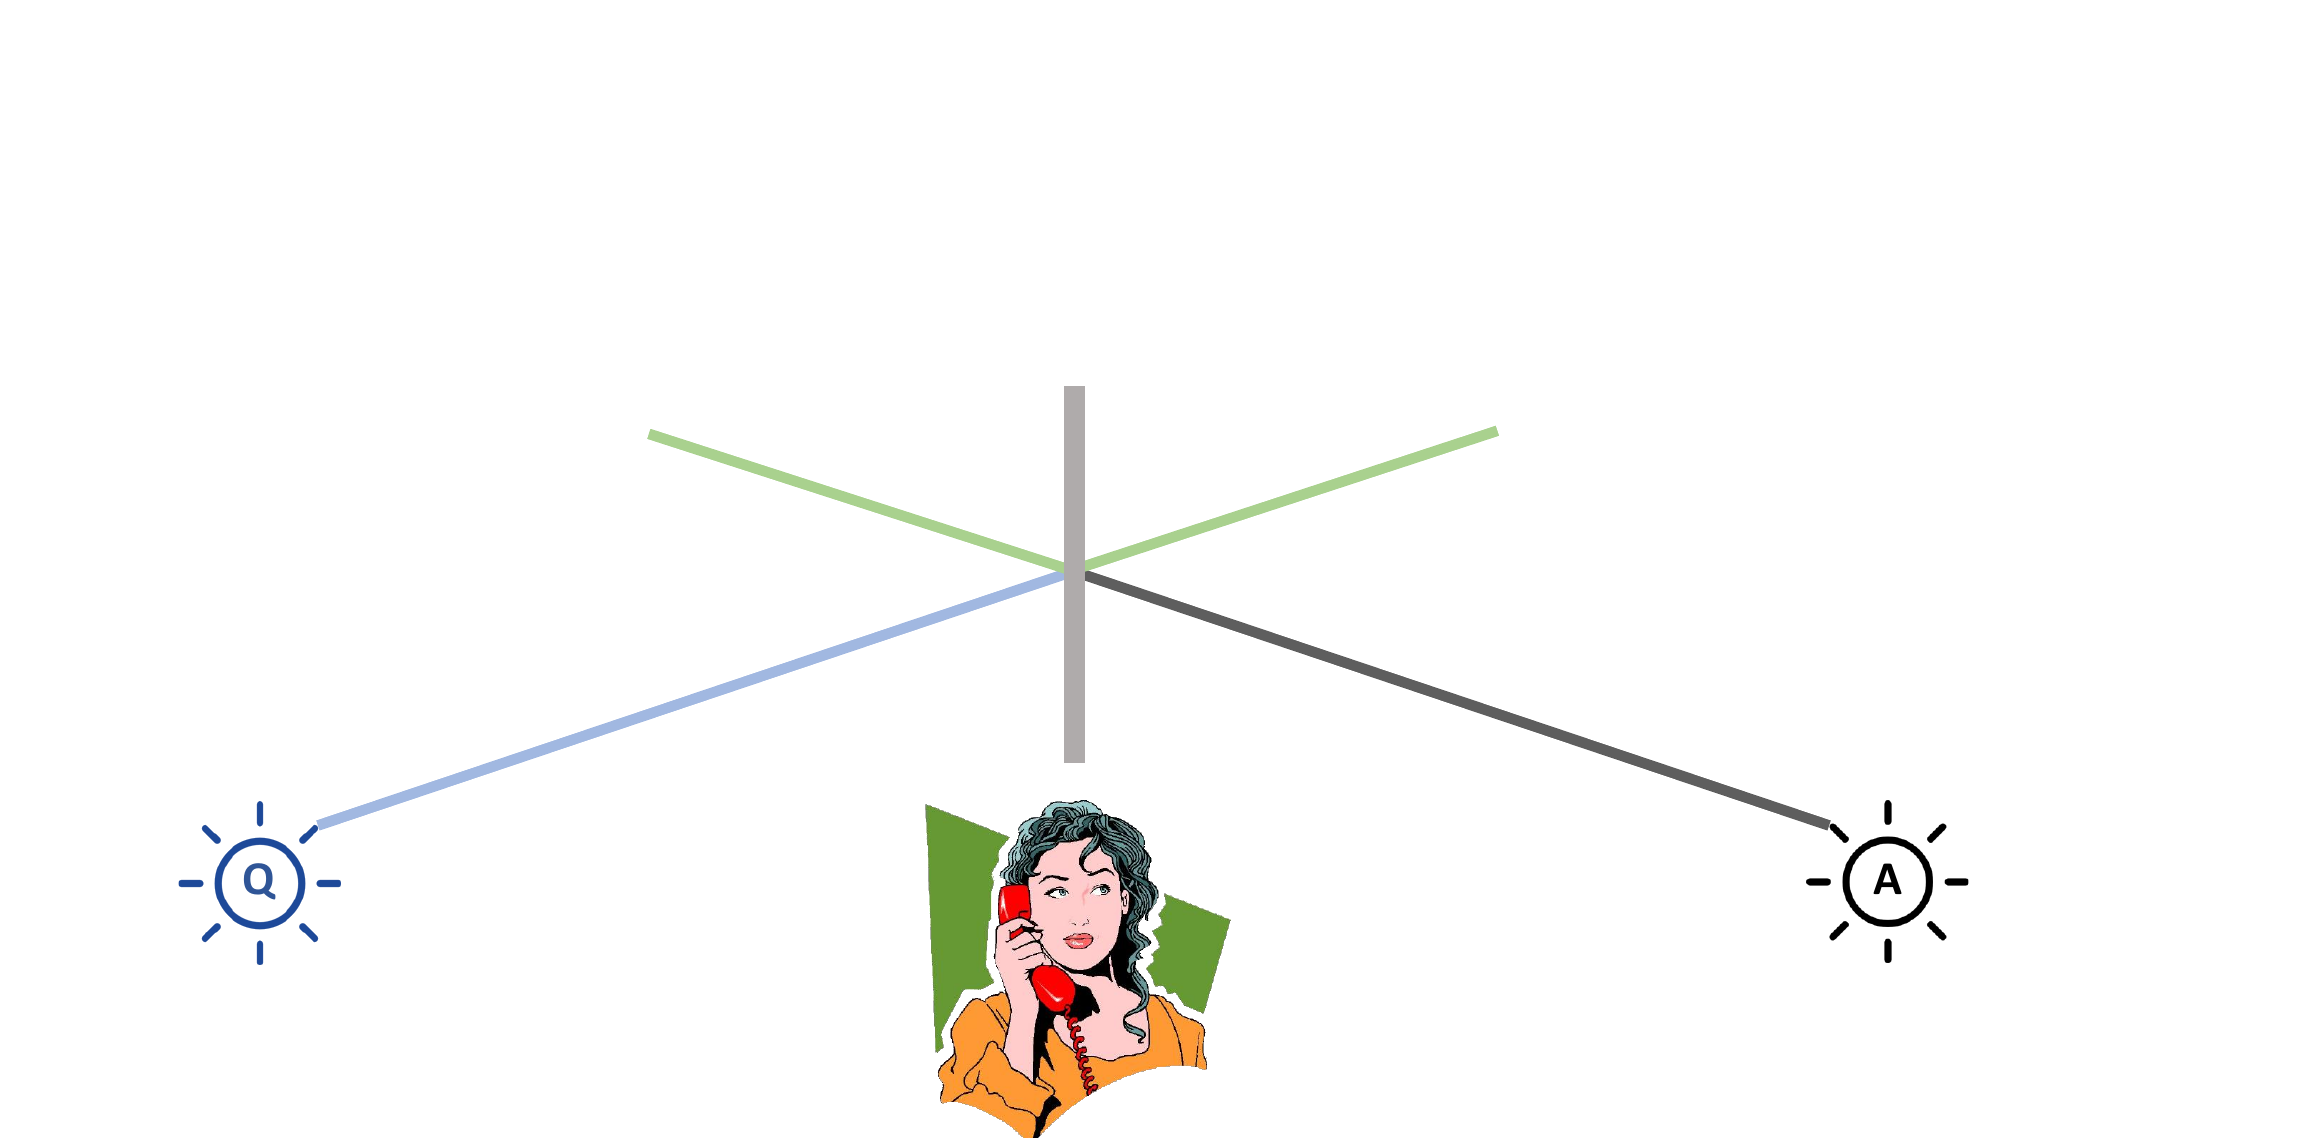
\includegraphics[scale=0.75]{figures/Teleportation/frame_12.png}}
\end{frame}

\begin{frame}
	\makebox[0pt][l]{\hspace{-2em}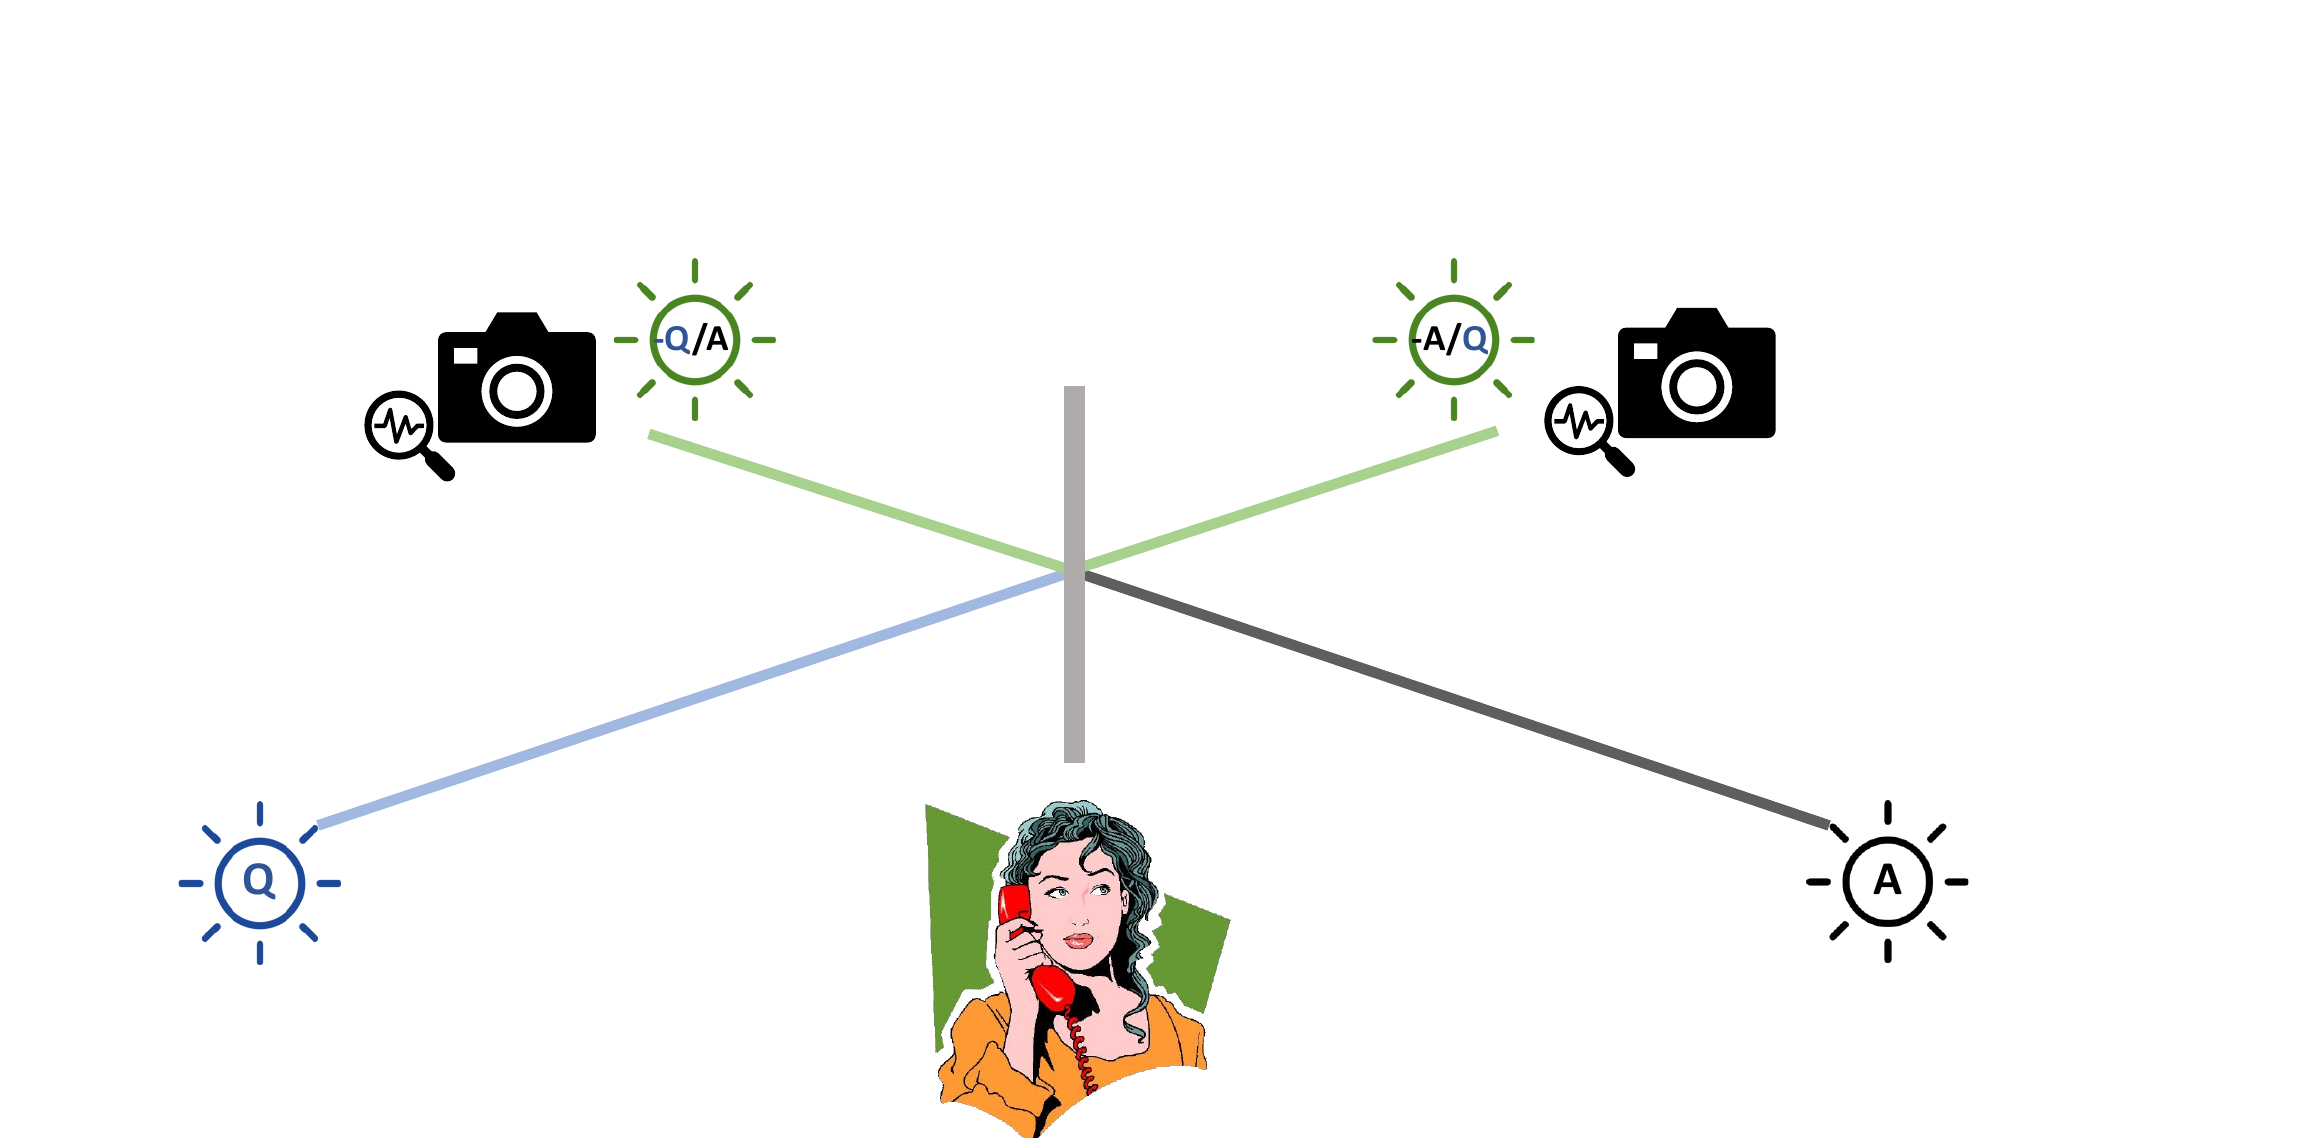
\includegraphics[scale=0.75]{figures/Teleportation/frame_13.png}}
\end{frame}

\begin{frame}
	\makebox[0pt][l]{\hspace{0em}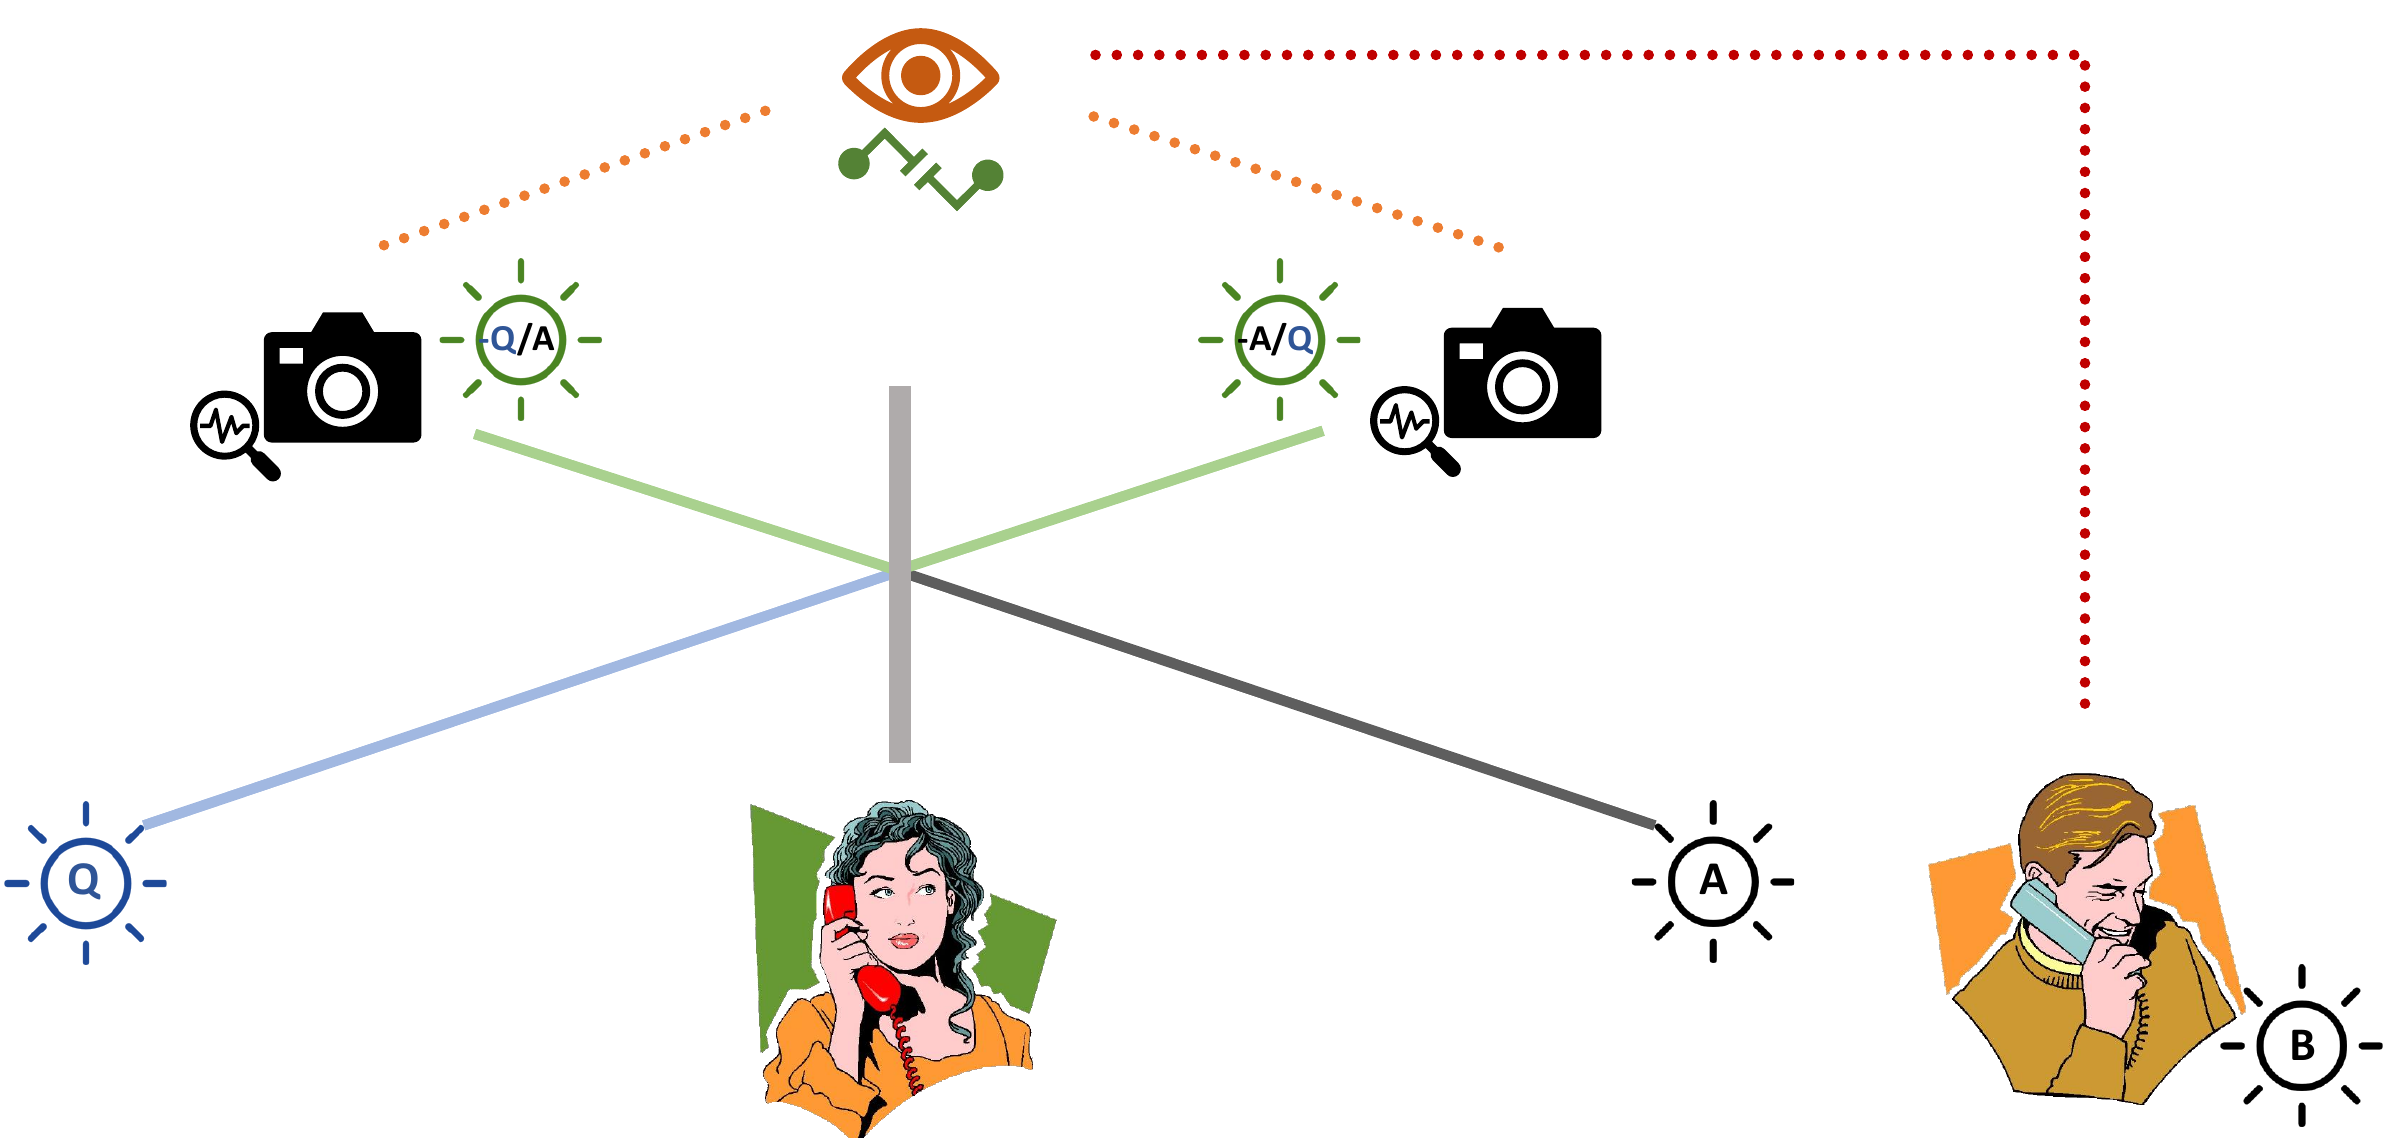
\includegraphics[scale=0.6]{figures/Teleportation/frame_14.png}}
\end{frame}

\begin{frame}
	\makebox[0pt][l]{\hspace{0em}\includegraphics[scale=0.6]{figures/Teleportation/frame_15.png}}
\end{frame}
